\documentclass[11pt]{memoir}

\usepackage{vinaya-class-notes}

\title{Vinaya Class Notes}
\author{The Bhikkhu Saṅgha}

\hypersetup{
  pdftitle={\thetitle},
  pdfauthor={\theauthor},
  pdfcopyright={Copyright (C) \the\year, \theauthor},
  pdfsubject={buddhism, vinaya},
  pdfkeywords={buddhism, vinaya},
  pdflicenseurl={https://creativecommons.org/licenses/by-nc-nd/4.0/},
  pdfcontacturl={https://vinaya-class.github.io/},
  pdflang={en},
}

\begin{document}

\frontmatter

\vspace*{-2cm}

{\centering%

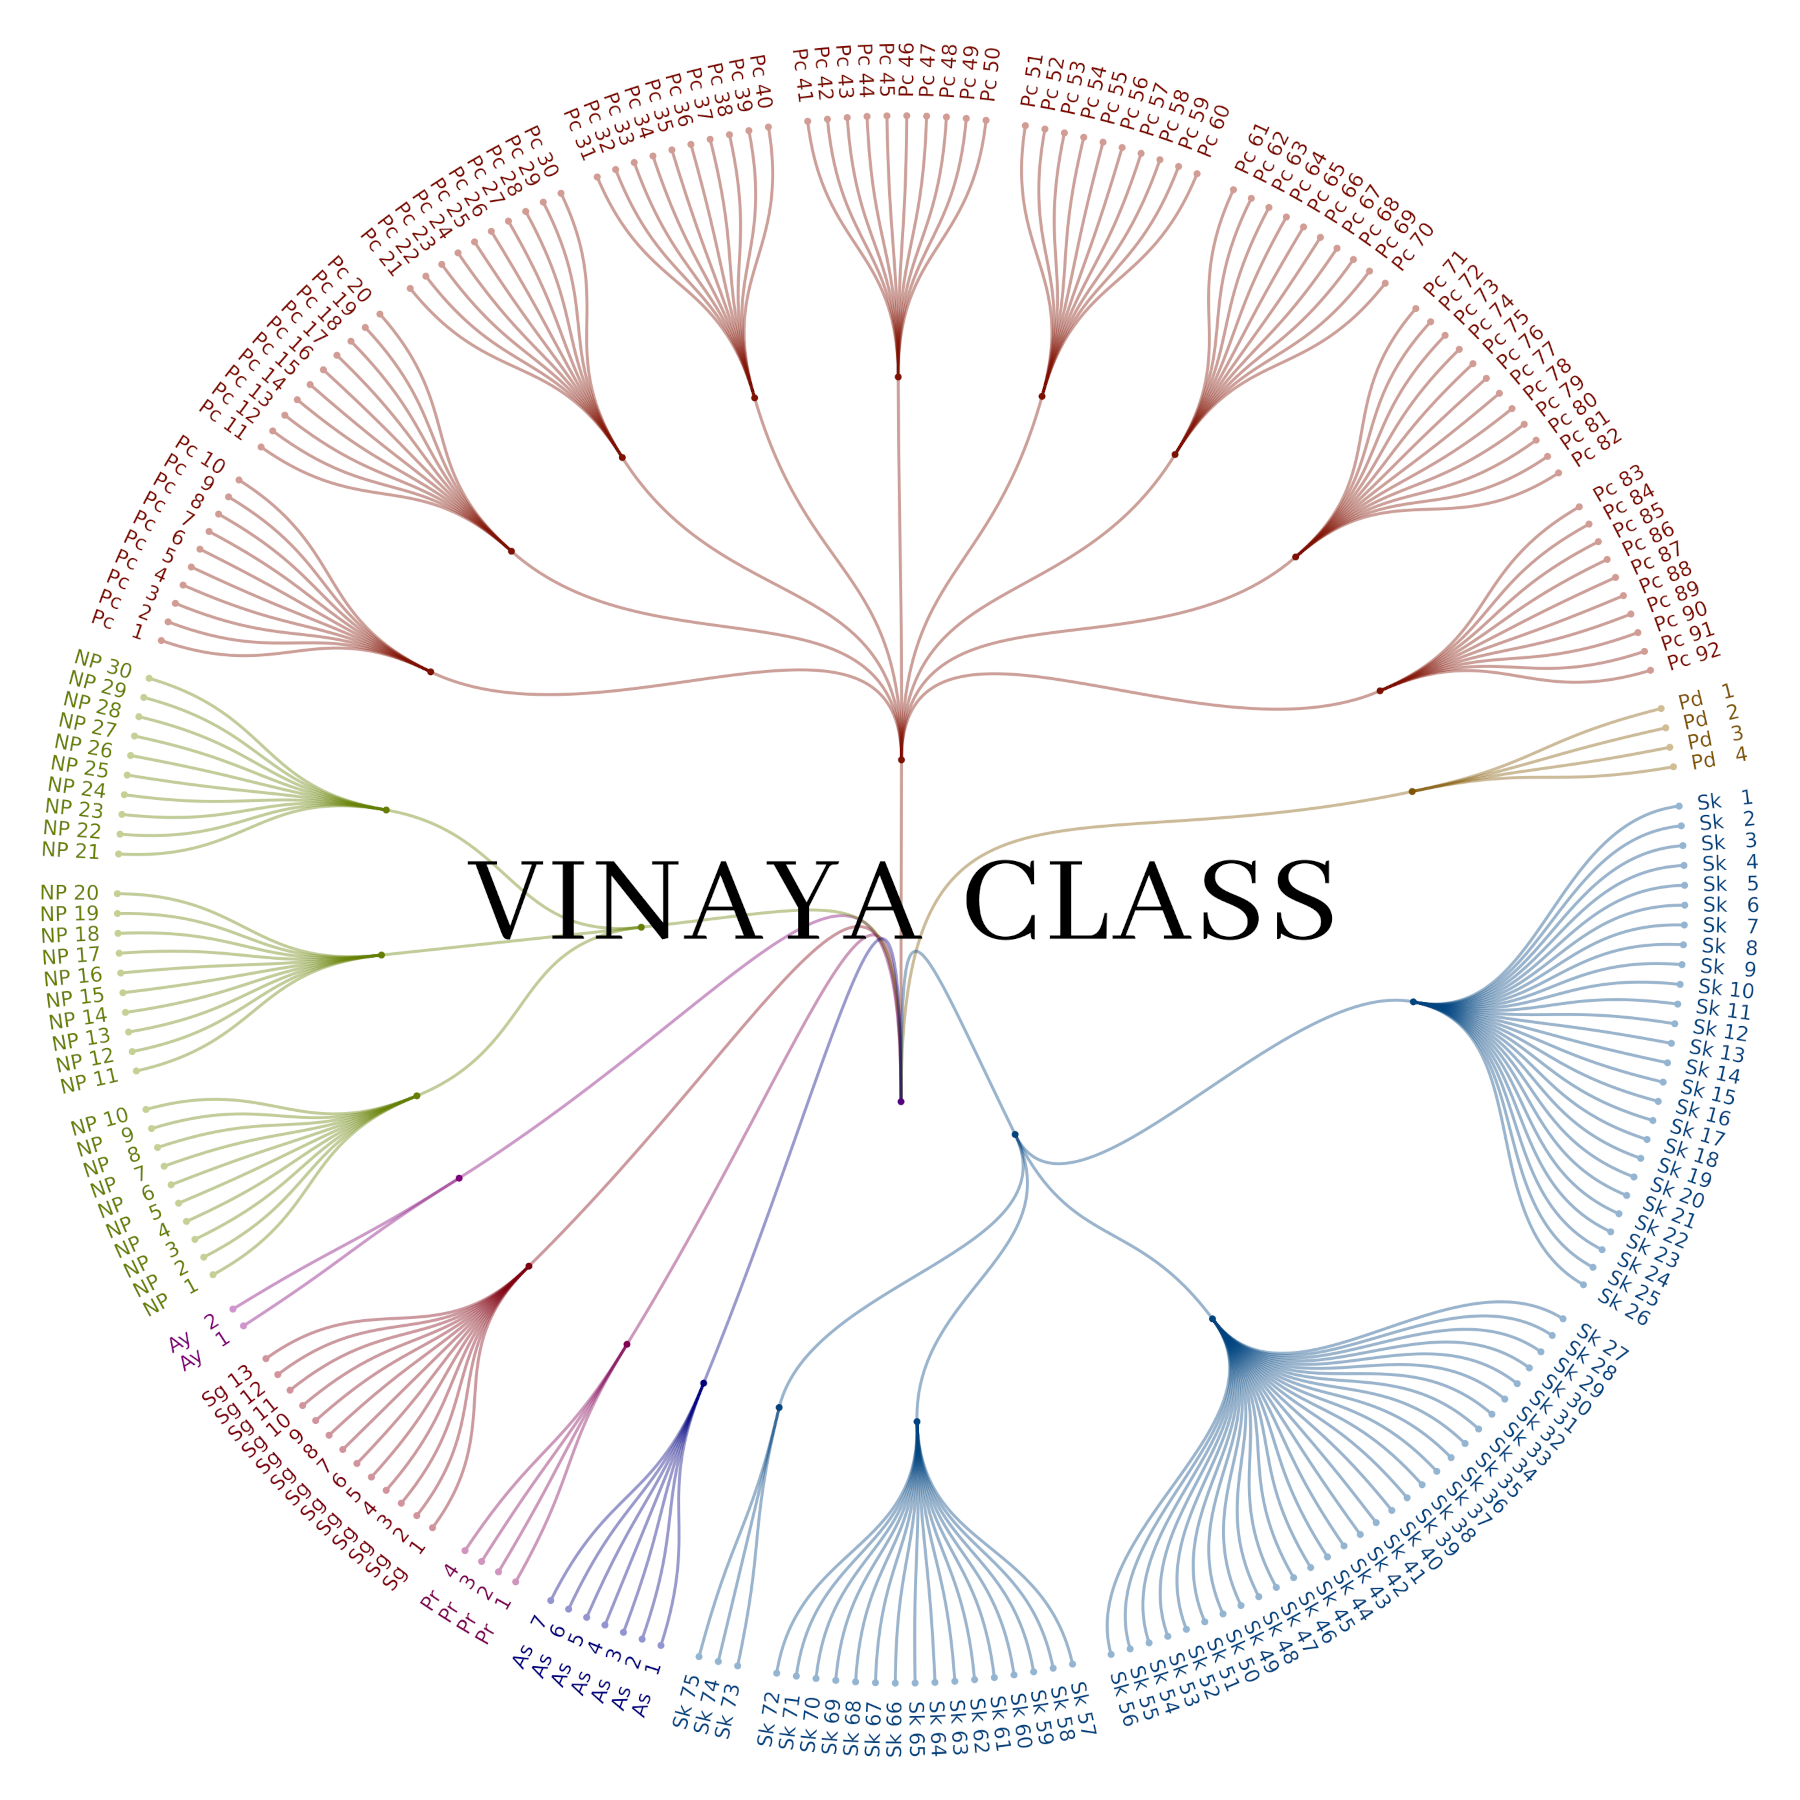
\includegraphics[width=10cm]{../../src/includes/figures/vinaya-class-title.w1800.png}

\href{https://vinaya-class.github.io}{https://vinaya-class.github.io}

{\scshape\small last updated on}\\
\today

}

\tableofcontents*

\chapter{Introduction}
\renewcommand*{\theChapterTitle}{Introduction}

\begin{exam}{\autoExamName}

\begin{problem}

  How can a bhikkhu determine if modern items (e.g. credit cards, sun glasses) are allowable or not?

  \bigskip

  \begin{answers}{1}
    \bChoices
    \Ans0 Discuss with the community and create a new rule\eAns
    \Ans0 Follow local cultural examples\eAns
    \Ans1 Discuss and follow the Four Great Standards\eAns
    \Ans0 One cannot know for sure what the Buddha's intentions were\eAns
    \eChoices
  \end{answers}

  \begin{solution}
    Suitable protocol for a community to discuss how to apply the Four Great
    Standards and agree on the accepted standards.
  \end{solution}

\end{problem}

\problemDivide

\begin{problem}

  A bhikkhu is visiting a friend who asks if it's all right for them to eat a
  pizza in the evening. The bhikkhu says it's fine by him, and they eat the pizza.
  \emph{Is this an offence?}

  \bigskip

  \begin{answers}{1}
    \bChoices
    \Ans0 No, because they are not in the monastery\eAns
    \Ans0 No, but there is a partial offence\eAns
    \Ans0 Usually it is, but it can depend on the situation\eAns
    \Ans1 Yes, it is a pācittiya offence\eAns
    \eChoices
  \end{answers}

  \bigskip

  \textbf{Discussion:} How does one determine whether there is full offence of a
  rule? What happens when not all factors are fulfilled for an offence?

  \begin{solution}
    Consider which of the five factors are fulfiled in the situation.
  \end{solution}

\end{problem}

\problemDivide

\begin{problem*}

  Match the type of offence with its description.

  \bigskip

  \begin{multicols}{2}

    \begin{parts}

    \item \fillin{2cm}{\ref{parajika}} pārājika
    \item \fillin{2cm}{\ref{sanghadisesa}} saṅghādisesa
    \item \fillin{2cm}{\ref{thullacaya}} thullacāya
    \item \fillin{2cm}{\ref{pacittiya}} pācittiya
    \item \fillin{2cm}{\ref{nissaggiya}} nissaggiya pācittiya
    \item \fillin{2cm}{\ref{dukkata}} dukkaṭa

    \columnbreak

    \bMatchChoices

    \item\label{thullacaya} grave offence
    \item\label{parajika} defeat
    \item\label{pacittiya} offence to be confessed
    \item\label{dukkata} wrong-doing
    \item\label{nissaggiya} involving forfeiture
    \item\label{sanghadisesa} involving community meetings

    \eMatchChoices
      
    \end{parts}
    
  \end{multicols}

  \bigskip

  \textbf{Discussion:} Advice on restoring one's faith after breaking a rule or
  having done something regrettable.

  \begin{solution}
    The classes of offences are: (1) pārājika, (2) saṅghādisesa, (3) thullacāya,
    (4) pācittiya, (5) nissaggiya pācittiya, (6) dukkaṭa.
  \end{solution}

\end{problem*}

\problemDivide

\begin{problem*}

  \begin{parts}

  \item Ignoring a \emph{sekhiya} etiquette rule out of disrespect for the
    training is\ldots

    \begin{answers}{4}
      \bChoices
      \Ans1 a wrong-doing\eAns
      \Ans0 to be confessed\eAns
      \Ans0 involves community meetings\eAns
      \Ans0 negligible, \emph{abbohārika}\eAns
      \eChoices
    \end{answers}

  \item Probation is a procedure following a \ldots{} offence.

    \begin{answers}{4}
      \bChoices
      \Ans0 pārājika\eAns
      \Ans1 saṅghādisesa\eAns
      \Ans0 pācittiya\eAns
      \Ans0 dukkaṭa\eAns
      \eChoices
    \end{answers}

  \end{parts}
  
  \bigskip

  \begin{solution}
    Mānatta is the penance, parivāsa is the probation procedure following a saṅghādisesa offence.
  \end{solution}

\end{problem*}

%\clearpage

\begin{problem*}

  \textbf{True} or \textbf{False}.

  \bigskip

  \begin{parts}

  \item \TF{F} Breaking a rule is always an offence for a bhikkhu, even if he doesn't
    remember the rule.

    \bigskip

    \textbf{Discussion:} Consider the case when he remembers, but goes ahead because the job has to be finished today.
    What is the proper protocol for him to follow?

  \item \TF{F} One of the Four Great Standards is that if it is not already allowed,
    but doesn't follow what is desirable, then it is allowable.

  \item \TF{F} During his upasampada, the candidate chants several lines of the
    ceremony incorrectly, therefore his ordination is invalid.

    \bigskip

    \textbf{Discussion:} What is essential for a valid bhikkhu upasampada?
    
  \item \TF{F} A young man (over 20) receives upasampada. He has concealed that
    he has to pay back his student loan, therefore his ordination is invalid.

  \item \TF{F} A bhikkhu's \emph{mentor} and \emph{preceptor} cannot be the same
    person.

  \item \TF{F} A bhikkhu complains about the monastic life and says, `Who am I kidding? Really,
    I want to disrobe.' After this statement he is no longer a bhikkhu.

    \bigskip

    \textbf{Discussion:} What are the factors of the disrobing procedure?

  \item \TF{F} A bhikkhu can request a \emph{baisuddhi} document when he arrives in Thailand.

    \bigskip

    \textbf{Discussion:} What is a \emph{baisuddhi}, who issues it, and what happens if you don't have one in Thailand?

  \item \TF{T} The community may decide to give a bhikkhu a new robe from the stores without formal \emph{sanghakamma}. 

    \bigskip

    \textbf{Discussion:} What are the steps of formal \emph{sanghakamma}?

  \end{parts}

\end{problem*}

\problemDivide

\begin{problem}

  The abbot of a monastery tells the community that in this monastery, the
  standard is that the last person finishing the meal must always empty the
  water from the spittoons and put away the seats. One monk, being in a hurry,
  doesn't do so and mosquitoes start breeding in the spittoon water. Are there
  offences?

  \bigskip

  \begin{answers}{4}
    \bChoices
    \Ans0 pārājika\eAns
    \Ans1 pācittiya\eAns
    \Ans0 dukkaṭa\eAns
    \Ans0 no offences\eAns
    \eChoices
  \end{answers}

\end{problem}

\bigskip

\textbf{Discussion:} What are some examples of local standards, or \emph{korwat}
rules? Cf. MN 48, Uda 4.5, Mv X on disputes at Kosambī. The Buddha then visits
the park where Ven. Anuruddha, Nandiya and Kimbila were living in harmony,
blending as `milk and water' (MN 31).

\problemDivide

\begin{problem}

  A bhikkhu lives alone in an accomodation on the property of his supporters. Some of
  his visitors consider him very accomplished and wish to join the monastic practice.
  What are the type of ordinations he can he give them?

  \bigskip

  \begin{manswers}{4}
    \bChoices
    \Ans0 bhikkhu\eAns
    \Ans1 samanera\eAns
    \Ans1 anagārika\eAns
    \Ans0 being alone, he can't ordain them\eAns
    \eChoices
  \end{manswers}

\end{problem}

\bigskip

\textbf{Discussion:} Who can act as a preceptor \emph{upajjhāya} to ordain bhikkhus?

\end{exam}



\mainmatter

\chapter{Killing and Harming}

\begin{itemize}
\tightlist
\item
  \textbf{Pr 3,} Killing a human being
\item
  \textbf{Pc 61,} Killing an animal
\item
  \textbf{Pc 20,} Pouring water containing living beings
\item
  \textbf{Pc 62,} Drinking water containing living beings
\item
  \textbf{Pc 10,} Digging soil
\item
  \textbf{Pc 11,} Damaging living plants or seeds
\end{itemize}

\section{Pr 3, Killing a human being}

\includemap{../../src/includes/mindmaps/pr-3.png}

\textbf{Origin:} bhikkhus develop aversion to the body and kill
themselves or ask an assassin to kill them.

Recommending death or euthanasia can be \textbf{parajika} if the
instruction is followed. Hinting fulfils effort, such as ``death would
be better for you''.

A human being is regarded as such from the time when the `being to be
born' is established in the womb. This is an uncertain time, sometime
after conception during embryo development. The embryo can't develop
otherwise.

\clearpage

\begin{quote}
``If consciousness were not to descend into the mother's womb, would
name-and-form take shape in the womb?''

``No, lord.''

``If, after descending into the womb, consciousness were to depart,
would name-and-form be produced for this world?''

``No, lord.''

``If the consciousness of the young boy or girl were to be cut off,
would name-and-form ripen, grow, and reach maturity?''

``No, lord.''

(\href{https://www.accesstoinsight.org/tipitaka/dn/dn.15.0.than.html}{DN
15})
\end{quote}

\section{Pc 61, Killing an animal}

Giving an order fulfils effort.

\textbf{Result} is a factor.

Doesn't include animals smaller than visible to the naked eye. Doesn't
include accidents (sweeping). No room for `phrasing it right'.

Origin: Ven. Udayin is killing crows by shooting them with arrows,
cutting their heads off and putting them in a row on a stake. The Buddha
scolds him, ``How can you, foolish man, intentionally deprive a living
thing of life? \ldots{}''
(\href{https://suttacentral.net/pli-tv-bu-vb-pc61/en/horner}{Vibh. Pc
61})

Mercy killing by the owner, or euthanasia practices by vets fulfil
effort. Having a pet means responsibility.

Acting in doubt, going ahead anyway is dukkata. Such as when the bhikkhu
thinks that cleaning an item may or may not kill living beings. Trying
carefully not to kill insects while cleaning is not an offence.

\textbf{Perception} is a factor. Stepping on a twig with the intention
to crush a snake is dukkata.

\section{Pc 20, Pouring water containing living beings}

Knowing they will die from pouring it. It can also include knowingly
adding poisonous substances.

If the water doesn't contain living beings, but the bhikkhu thinks it
does, pouring or using it is dukkata.

Giving an order fulfils effort.

Result is not a factor. Doesn't include accidents.

Can't water plants if one plans to eat its fruit, but may indicate it
for others.

Kutis may use small gutters as water moats around the stilts to keep out
ants. One has to treat the water with household chemicals, otherwise
mosquitoes will breed in the water.

\section{Pc 62, Drinking water containing living beings}

\enlargethispage{\baselineskip}

Knowing they will die from drinking it, even accidentally.

Using water strainers or robe. Determining a corner of the sanghati as a
water-filter.

Result is not a factor.

\clearpage

\section{Pc 10, Digging soil}

\begin{multicols}{2}

\textbf{Origin:} relates to the ancient belief that soil is alive, and
loses life when dug up.

\textbf{Object:} `genuine' soil.

\emph{Not} genuine soil:

\begin{itemize}
\tightlist
\item
  dust from wind erosion
\item
  pure or mostly rock, stones, gravel, sand are never `genuine' soil
\item
  burnt or already dup up soil is not `genuine' until rained on for four
  months
\end{itemize}

If someone digs up the soil, a bhikkhu may shovel it into a wheelbarrow
without offence.

\textbf{Effort:} Digging, burning, making a hole, or giving command to
do it.

Putting tent pegs in the ground is to be confessed.

\columnbreak

\textbf{Non-offenses:}

\begin{itemize}
\tightlist
\item
  unknowingly, unthinkingly, unintentionally
\item
  indicating a general need or task
\item
  asking for clay or or soil
\item
  digging a trapped person or animal out
\end{itemize}

Allowance to indicate a need or general task to a lay person by
``wording it right (\emph{kappiya-vohāra},''allowable expression," or
``wording it right'').

A specific command would be an offense (`dig a hole here'), but an
indication (`dig a hole') of a desire or intent would not (`it would be
good to have a hole for this post').

\end{multicols}

\section{Pc 11, Damaging living plants or seeds}

\begin{multicols}{2}

\textbf{Origin:} a bhikkhu cuts down a tree where a deva was living. The
rule is formed later, when people complained of the bhikkhus mistreating
one-facultied life.

\textbf{Object:} Living plant or seed. Lower plant life (i.e.~mold,
algae, fungi) is not included.

\textbf{Effort:} cutting, breaking, cooking, or getting others to do it.

\textbf{Fruit with seeds:} allowance to make allowable (kappiyam). Fruit
can be kappied in one ``heap''.

\columnbreak

To `kappi' fruit is about the feelings of the donor, not killing the
fruit or transfering kamma.

Knowingly eating un-kappied seeds is dukkata.

\textbf{Non-offenses:}

\begin{itemize}
\tightlist
\item
  unknowingly, unthinkingly, unintentionally
\item
  asking a lay person for flowers etc. in general, or indicating a
  general task
\item
  removing branches or leaves which are already dead
\item
  can cut a trapped person or animal out
\item
  counter-fire
\end{itemize}

\end{multicols}
\par
\enlargethispage{2\baselineskip}

\textbf{Note:} Pc 10 and Pc 11 prevents bhikkhus from engaging in
agriculture, which is probably part of the intended results, although
not their direct origin.


\chapter{2. Stealing}
\renewcommand*{\theChapterTitle}{2. Stealing}

\begin{exam}{\autoExamName}

\begin{problem*}

  Are there offences?

\begin{parts}

  \item A bhikkhu sneaks into the kitchen and eats an apple.

  \bigskip

  \begin{answers}{5}
    \bChoices
    \Ans0 pārājika\eAns
    \Ans0 thullacāya\eAns
    \Ans1 pācittiya\eAns
    \Ans0 dukkaṭa\eAns
    \Ans0 no offences\eAns
    \eChoices
  \end{answers}

  \bigskip

  \begin{solution}
    Pācittiya for eating unoffered food, another pacittiya if eating in the
    wrong time. Stealing doesn't apply if the contents of the kitchen are
    considered Sangha property.
  \end{solution}

  \item The same bhikkhu sees a wallet left on the kitchen counter and picks it
    up, hoping to find money in it. He only finds ID cards, so he takes the wallet
    to the monk's office for safe-keeping.

  \bigskip

  \begin{answers}{5}
    \bChoices
    \Ans0 pārājika\eAns
    \Ans1 thullacāya\eAns
    \Ans0 pācittiya\eAns
    \Ans0 dukkaṭa\eAns
    \Ans0 no offences\eAns
    \eChoices
  \end{answers}

  \begin{solution}
    Stealing is complete as soon as picking it up. Thullacāya, because there are
    no valuables.
  \end{solution}

  \bigskip

  \item A man gives a bhikkhu a new phone as a gift. He says he was able to get it very cheaply.
  The bhikkhu doesn't know that the phone comes from a batch stolen from the factory. 

  \bigskip

  \begin{answers}{5}
    \bChoices
    \Ans0 pārājika\eAns
    \Ans0 thullacāya\eAns
    \Ans0 pācittiya\eAns
    \Ans0 dukkaṭa\eAns
    \Ans1 no offences\eAns
    \eChoices
  \end{answers}

  \begin{solution}
    There is no offense assigned for receiving stolen goods, even knowingly.
  \end{solution}

  \bigskip

  \item A bhikkhu is visiting a monastery. He is frustrated that he is not given
    the WiFi password. He uses a program on his laptop to break the WiFi encryption
    and steal the password anyway.

  \bigskip

  \begin{answers}{5}
    \bChoices
    \Ans0 pārājika\eAns
    \Ans0 thullacāya\eAns
    \Ans0 pācittiya\eAns
    \Ans1 dukkaṭa\eAns
    \Ans0 no offences\eAns
    \eChoices
  \end{answers}

  \begin{solution}
    Dukkaṭa for a broken promise. `Stealing a password' is colloquial language
    for `copying without permission'.
  \end{solution}

  \bigskip

  \textbf{Discussion:} What if this is in a hotel where they charge for WiFi access?

  \begin{solution}
    Dukkaṭa for a broken promise, pacittiya if deceit is involved. Using services without permission is not stealing.
  \end{solution}

  \bigskip

  \item A bhikkhu is preparing to visit England. A visitor at the monastery asks
    him to carry an expensive audio recorder with him and give it to his friend in
    England. The bhikkhu decides to keep the recorder.

  \bigskip

  \begin{answers}{5}
    \bChoices
    \Ans0 pārājika\eAns
    \Ans0 thullacāya\eAns
    \Ans0 pācittiya\eAns
    \Ans1 dukkaṭa\eAns
    \Ans0 no offences\eAns
    \eChoices
  \end{answers}

  \begin{solution}
    Parajika if the recorder is seen as the friend's property.
    Dukkaṭa for a broken promise.

    Make sure to clarify intentions, ask again for
    clear statements if necessary.

    `I give this to you, please give it to X' -- he is given ownership of the
    item, and \emph{promises} to give it to X.

    `This is my friend's recorder, please take it to him' -- he is not given
    ownership, if he keeps it, the penalty is parajika.
  \end{solution}

  \bigskip

  \item A bhikkhu receives a bag of expensive sweets on alms-round from a lady, who
  says, `I bought these for the abbot'. The bhikkhu eats a bit from it before giving it
  to the abbot.

  \bigskip

  \begin{answers}{5}
    \bChoices
    \Ans0 pārājika\eAns
    \Ans1 thullacāya\eAns
    \Ans0 pācittiya\eAns
    \Ans1 dukkaṭa\eAns
    \Ans0 no offences\eAns
    \eChoices
  \end{answers}

  \begin{solution}
    Thullacāya because he only eats a small bit, not the whole bag. Dukkaṭa for a broken promise.
  \end{solution}

  \bigskip

  \item A senior bhikkhu places a bowl under shared ownership (\emph{vikappana}) with a samanera.
  He tells the bhikkhu that he may take it anytime when he needs it, and keeps the bowl in his kuti.
  A year later, the samanera is now a junior bhikkhu.
  The senior bhikkhu takes the bowl from the kuti when the junior bhikkhu is not there.

  \bigskip

  \begin{answers}{5}
    \bChoices
    \Ans0 pārājika\eAns
    \Ans0 thullacāya\eAns
    \Ans0 pācittiya\eAns
    \Ans0 dukkaṭa\eAns
    \Ans1 no offences\eAns
    \eChoices
  \end{answers}

  \begin{solution}
    No offense for taking items on trust when there has been a previous
    arrangement. In this case, no offense for using a \textit{vikappana} item:
    the \emph{vikappana} is automatically rescinded when items are taken on
    trust.
  \end{solution}

  \item A bhikkhu is visiting a monastery and makes a long phone call. The call
  costs €100. The resident monks discover it on the bill and ask if
  anyone knows about this call. He remains silent.

  \bigskip

  \begin{answers}{5}
    \bChoices
    \Ans0 pārājika\eAns
    \Ans0 thullacāya\eAns
    \Ans1 pācittiya\eAns
    \Ans1 dukkaṭa\eAns
    \Ans0 no offences\eAns
    \eChoices
  \end{answers}

  \begin{solution}
    Dukkaṭa for the broken promise (using unauthorized services). Pācittiya for deceit.
  \end{solution}

\end{parts}

\end{problem*}

\end{exam}

\section*{Discussion}

How is it possible for a bhikkhu to steal from the Sangha?

\bigskip

A bhikkhu drives away with the monastery car and never comes back.
What are the consequences?


\chapter{3. Sexual Conduct}
\renewcommand*{\theChapterTitle}{3. Sexual Conduct}

\begin{exam}{\autoExamName}

\begin{problem}

  A bhikkhu is staying at the apartment of a friend, where they organize a small
  gathering, and they start drinking alcohol. The bhikkhu gets drunk, and
  eventually he goes to bed in his room. He wakes up, and finds a woman's
  underwear in his bed, with a note saying `love and kisses', plus a used
  condom.

  Is the bhikkhu pārājika? 

  \bigskip
 
  \begin{answers}{1}
    \bChoices
    \Ans0 No, because he was drunk\eAns
    \Ans0 No, if he was practising trantric freedom and compassion\eAns
    \Ans1 Yes, since there is clear evidence of intercourse\eAns
    \Ans0 Yes, even if he can't remember anything\eAns
    \eChoices
  \end{answers}

  \bigskip

  \textbf{Discussion:} What if he convinces himself that he is pārājika, but
  later finds out that they had played a prank on him?
  
\end{problem}

\problemDivide

\begin{problem}

  Mark the factors which, under \textit{Sg 1}, commit a \textit{thullacāya} offence.

  \begin{answers}{6}
    \bChoices
    \Ans0 object\eAns
    \Ans0 perception\eAns
    \Ans1 intention\eAns
    \Ans1 effort\eAns
    \Ans0 result\eAns
    \eChoices
  \end{answers}

  \bigskip

  \textbf{Discussion:} describe such a situation.

\end{problem}

\problemDivide

\begin{problem*}

  Are there offences?

\begin{parts}

\item
  A women asks to speak with a bhikkhu.
  It is a hot day and she is dressed quite openly.
  For the rest of the day, he continues fantasising about her.

  \bigskip

  \begin{answers}{6}
    \bChoices
    \Ans0 pārājika\eAns
    \Ans0 saṅghādisesa\eAns
    \Ans0 thullacāya\eAns
    \Ans0 pācittiya\eAns
    \Ans0 dukkaṭa\eAns
    \Ans1 no offences\eAns
    \eChoices
  \end{answers}

  \bigskip

  \item Later, the bhikkhu recollects the meeting, starts rubbing himself, and causes an emission.

  \bigskip

  \begin{answers}{6}
    \bChoices
    \Ans0 pārājika\eAns
    \Ans1 saṅghādisesa\eAns
    \Ans0 thullacāya\eAns
    \Ans0 pācittiya\eAns
    \Ans0 dukkaṭa\eAns
    \Ans0 no offences\eAns
    \eChoices
  \end{answers}

  \bigskip

  \textbf{Discussion:} asking women to cover themselves when they come to a
  meeting in what is a normal dress for them.

  \bigskip

\end{parts}

\end{problem*}

\end{exam}

\chapter{Lustful Conduct}

\begin{itemize}
\tightlist
\item
  \textbf{Sg 2,} Lustful contact with a woman
\item
  \textbf{Sg 3,} Speaking lewd words to a woman
\item
  \textbf{Sg 4,} Praising sexual intercourse as gift
\item
  \textbf{Pc 7,} Teaching more than six sentences
\end{itemize}

\section{Sg 2, Lustful contact with a woman}

\begin{multicols}{2}

Origin: Ven. Udayin disturbing a bhrahmin's wife while they are visiting
him.

\textbf{Object:} a living woman, ``even one born on that day.'' Body,
hand, limbs, a lock of hair, etc.

\textbf{Perception:} perceiving her to be a woman.

\textbf{Intention:} impelled by lust, any state of passion, desire to
enjoy the contact. Can be an extended period of desire, or a momentary
attraction.

Contact out of filial affection for family members is a dukkata.

\textbf{Effort:} physical contact.

Items she is wearing are direct contact.

Indirect contact:

\begin{itemize}
\tightlist
\item
  touching a item which she is holding: thullacaya
\item
  touching her with an item one is holding: thullacaya
\item
  item to item: dukkata
\item
  tossing: dukkata
\item
  shaking sth. she is standing on: dukkata
\end{itemize}

Passive contact:

Contact while trying to shake her off is not an offense.

If the bhikkhu's aim is to partake, the offense is sanghadisesa.

\subsection{Non-offenses}

\begin{itemize}
\tightlist
\item
  unintentionally
\item
  unthinkingly
\item
  unknowingly
\item
  the bhikkhu doesn't give his consent
\item
  no desire for the contact
\item
  has desire, but makes no effort
\end{itemize}

\end{multicols}

\section{Sg 3, Speaking lewd words to a woman}

\begin{multicols}{2}

Wanting to enjoy saying something lewd. Directly referencing \emph{her}
genitals, anus, or her performing sexual intercourse. Slang, euphemisms,
non-verbal gestures fulfill effort.

\textbf{Object:} Any woman who recognizes lewd comments.

May not know: too young, too innocent or retarded, or doesn't know the
language.

\textbf{Perception:} The bhikkhu perceives her to be a woman.

\textbf{Intention:} Impelled by lust. The minimum lust is wanting to
enjoy saying something lewd.

\begin{itemize}
\tightlist
\item
  not necessary to have desire to have sex with her
\item
  statements in anger come under Pc 2 instead
\end{itemize}

\textbf{Effort:} Praising, criticizing, asking, etc. referencing her
genitals, anus, or her performing sexual intercourse.

\begin{itemize}
\tightlist
\item
  direct mention of above
\item
  indirect references, slang, euphemisms, non-verbal gestures fulfill
  effort
\end{itemize}

Another person's private parts don't fulfill effort.

\textbf{Result:} The woman immediately understands.

If she only understands later:

\begin{itemize}
\tightlist
\item
  \emph{thullacaya} if it was a direct reference
\item
  \emph{dukkata} if it was indirect
\end{itemize}

\subsection{Non-offenses}

\begin{itemize}
\tightlist
\item
  speech aiming at spiritual welfare, if not out of lust
\item
  the bhikkhu doesn't intend to be lewd, but the woman takes it as lewd
\end{itemize}

\end{multicols}

\section{Sg 4, Praising sexual intercourse as gift}

A variation on lewd speech.

Directly countering the notion that ``giving'' sex as a spiritual gift
brings good karmic rewards.

Intention is fulfilled simply by the desire to enjoy making such remarks
in the presence of a woman, even if just to test her reactions.

\section{Pc 7, Teaching more than six sentences}

\begin{multicols}{2}

Origin: Ven. Udayin whispers Dhamma sentences in the ears of certain
women.

One should ask a man to chaperon when engaging in a conversation or
interview with women.

The rule is aimed at preventing a bhikkhu from using his knowledge of
Dhamma as a way of making himself attractive to a woman.

The rule aims to protect both the woman and the monk. In the origin
story, other women get jealous that Ven. Udayin didn't teach them
Dhamma.

Note that male doctors sometime refuse to see female patients without a
nurse present.

Other topics have no penalty, but indulging in `animal talk' with lay
people may result in censure, banishment or suspension on grounds of
`unbecoming assoication with householders' or `verbal frivolity.'

Also, observers might misinterpret the situation, best to ask someone to
chaperon.

Private conversations in general are treated in Pc 44, Pc 45, Ay 1, Ay
2.

\columnbreak

\textbf{Object:} Any woman who recognizes lewd comments.

\textbf{Perception} is not a factor.

\textbf{Effort:} Teaching more than six sentences of Dhamma without a
knowledgeable man present.

\subsection{Non-offenses}

\begin{itemize}
\tightlist
\item
  if the woman changes position
\item
  talk on different occasions
\item
  addressing the next woman
\item
  teaching someone else, and the woman just listens in
\item
  teaching in response to questions from the woman
\end{itemize}

\end{multicols}


\chapter{Women 1}

\begin{itemize}
\tightlist
\item
  \textbf{Sg 5,} Conveying romantic messages
\item
  \textbf{Pc 6,} Lying down with a woman
\item
  \textbf{Pc 44,} Private secluded place
\item
  \textbf{Pc 45,} Unsecluded but private place
\item
  \textbf{Pc 67,} Travelling by arrangement with a woman
\end{itemize}

\includemap{../../src/includes/mindmaps/women.png}

\begin{quote}
``Lord, what course should we follow with regard to womenfolk?''

``Not-seeing, Ānanda.''

``But when there is seeing, lord, what course should be followed?''

``Not-addressing, Ānanda.''

``But when we are addressed, what course should be followed?''

``Mindfulness should be established, Ānanda.''

\emph{\href{https://www.dhammatalks.org/suttas/DN/DN16.html}{DN 16}}
\end{quote}

\section{Sg 5, Conveying romantic messages}

Origin: Ven. Udayin acts as a matchmaker between several families, some
of whom didn't even know each other before. For some matches they praise
him, for other matches they curse him. In one particular case they treat
the girl like a slave, who repeatedly sends unhappy messages back to her
family.
(\href{https://suttacentral.net/pli-tv-bu-vb-ss5/en/brahmali}{Vib. Ss.
5})

Only two factors: effort and object.

\textbf{Effort:} `Conveying' messages for any romantic purpose from a
momentary date to a wedding. Not business meetings.

\clearpage

Three stages:

\begin{itemize}
\tightlist
\item
  \emph{accepting} the request to convey a message
\item
  \emph{inquiring} at the second party
\item
  \emph{reporting} the response
\end{itemize}

Dukkata for any single stage, thullacaya for any two, sanghadisesa for
all three.

Carrying a letter without knowing the content doesn't fulfill effort.

Keeping email and phone contacts private. Nonetheless it fulfills
\emph{inquiring}.

\textbf{Object:} A man and a women who are not married to each other,
even if dealing with them via other people.

Reconciling a still married couple is not an offense. Reconciling a
divorced couple is sanghadisesa.

\enlargethispage{2\baselineskip}

\textbf{Non-offenses:} messages about non-romantic errands,
e.g.~community business, a shrine, a sick person.

`Being married' is clear in the case of a church- or civil marriage, or
if there had been some other formal civic arrangement. Other, more
vague, customary forms of living together, sharing a child, or long-term
relationships become difficult the determine.

\section{Pc 6, Lying down with a woman}

Origin: Ven. Anuruddha stays at the house of a wealthy woman for a
night. She approaches him, but he remains unmoved, and she leaves. There
was no offence, but the rule is established to avoid similar situations.

\textbf{Object:} Female human being, even a baby, one's relative or not.

\textbf{Effort:} in the instant one lies down in the same dwelling when
a woman is lying down.

Same dwelling: one ``enclosure''. Technically the same walls and roof,
but one may consider variations (private hospital rooms).

Intention is not a factor, pacittiya even if the bhikkhu doesn't know
about the woman.

Purpose: to avoid situations where people might think that one may have
commited serious offenses. Other people might see the situation and
rumors would be damaging.

Non-offenses for roofed but no walls (pavilion) or walled but not roofed
(corral), but a good idea to avoid nonetheless.

\section{Pc 44, Private secluded place}

Origin: Ven. Upananda sat down with the wife of a friend on a private
and concealed seat. Later, the husband complained and criticized him.
The Buddha rebuked Ven. Upananda, ``Foolish man, how can you sit in
private on a concealed seat with a woman? This will not give rise to
confidence in those without it\ldots{}''
(\href{https://suttacentral.net/pli-tv-bu-vb-pc44/en/brahmali}{Vibh. Pc.
44})

The bhikkhu sits with a woman at a secluded place, private to the eye
and ear, without another man present, aiming at privacy. Secluded enough
for parajika.

\textbf{Effort:} sitting or lying down on the same seat.

\subsection{Non-offences}

\vspace*{-0.5\baselineskip}
\enlargethispage{\baselineskip}

\begin{itemize}
\tightlist
\item
  if a knowledgeable man is present
\item
  if the woman entered the room later, and he didn't notice
\item
  either or both of them are standing
\end{itemize}

\section{Pc 45, Unsecluded but private place}

The bhikkhu sits with a woman at a private, but not secluded place, such
as an empty park, without another \emph{person} present. Secluded enough
for sanghadisesa.

\section{Pc 67, Travelling by arrangement with a woman}

Origin: a woman hears that a monk is going to a village and goes with
him. Later, the woman's husband heard about it and gave him a beating.

Purpose: to avoid people assuming the bhikkhu having an affair with the
woman.

In the monastery, female lay supporters often help with transport which
are arranged. This becomes casuse for concern when a bhikkhu arranges to
travel with the same woman again and again.

\textbf{Object:} Any woman who knows what is lewd.

\textbf{Perception} is not a factor.

\textbf{Effort:}

\begin{enumerate}
\def\labelenumi{\arabic{enumi}.}
\tightlist
\item
  having made an arrangement to travel together
\item
  they travel as arranged

  \begin{itemize}
  \tightlist
  \item
    time frame as arranged
  \item
    route or place of departure doesn't count
  \end{itemize}
\item
  from one village to another (half-yojana, 8km)
\end{enumerate}

\textbf{Making an arrangement:} both gives verbal or written assent to
the arrangement.

Giving assent in silence is not an offense.

\begin{itemize}
\tightlist
\item
  if the women doesn't respond: \emph{dukkata}
\item
  if the bhikkhu doesn't respond: no offense
\end{itemize}

\subsection{Non-offenses}

\begin{itemize}
\tightlist
\item
  coincidence: they happen to travel together
\item
  the woman proposes the arrangement, and the bhikkhu doesn't give
  \emph{verbal} assent
\item
  leaving at a significantly different time than as arranged
\item
  there are dangers
\end{itemize}

\subsection{Cases}

\begin{itemize}
\tightlist
\item
  public transport
\item
  private transport (Pc 44)
\end{itemize}

\clearpage

\begin{quote}
``But what, Master Gotama, is a gap, a break, a spot, a blemish of the
holy life?''

\begin{itemize}
\tightlist
\item
  "He does consent to being anointed, rubbed down, bathed, or massaged
  by a woman
\item
  he jokes, plays, and amuses himself with a woman
\item
  he stares into a woman's eyes
\item
  he listens to the voices of women outside a wall as they laugh, speak,
  sing, or cry
\item
  he recollects how he used to laugh, converse, and play with a woman
\item
  he sees a householder or householder's son enjoying himself endowed
  with the five strings of sensuality
\item
  he practices the holy life intent on being born in one or another of
  the deva hosts
\end{itemize}

``He enjoys that, wants more of that, and luxuriates in that. This is a
gap, a break, a spot, a blemish of the holy life. He is called one who
lives the holy life in an impure way, one who is fettered by the fetter
of sexuality. He is not freed from birth, aging, \& death, from sorrows,
lamentations, pains, griefs, \& despairs. He is not freed, I tell you,
from suffering \& stress.''

(\href{https://www.dhammatalks.org/suttas/AN/AN7_47.html}{AN 7.47})
\end{quote}


\chapter{Attainments}

\begin{itemize}
\tightlist
\item
  \textbf{Pr 4,} Lying about superior attainments
\item
  \textbf{Pc 8,} Telling unordained person about actual attainment
\end{itemize}

\includemap{../../src/includes/mindmaps/attainments.png}

\section{Pr 4, Lying about superior attainments}

Extreme case of lying (Pc 1).

Origin: During a period of drought and famine, certain bhikkhus praised
each other's false attainments to the lay people so that they may have a
comfortable Vassa.
(\href{https://suttacentral.net/pli-tv-bu-vb-pj4/en/brahmali}{Vibh. Pr
4})

\begin{quote}
How can you for the sake of your stomachs praise one another's
superhuman qualities to lay people? It would be better for your bellies
to be cut open with a sharp butcher's knife than for you to praise one
another's superhuman qualities to lay people.

Why is that? Because for that reason you might die or experience
death-like suffering, but you wouldn't because of that be reborn in a
bad destination. But for \emph{this} reason you might.
\end{quote}

\clearpage

Five great gangsters as bad monks:

\begin{enumerate}
\def\labelenumi{\arabic{enumi}.}
\tightlist
\item
  wanting to be honoured, revered and obtain gifts
\item
  learning the Buddha's teachings and taking it as his own
\item
  accusing a pure practitioner of the holy life of sexual intercourse
\item
  taking and using Sangha property to create a following among lay
  people
\item
  `But in this world this is the greatest gangster: he who untruthfully
  and groundlessly boasts about a superhuman quality. Why is that?
  Monks, you've eaten the country's almsfood by theft.'
\end{enumerate}

\textbf{Object:} superior human states which are not accessible to
mundane, ordinary people (\emph{puthujjana}). States are categorized in
three groups.

\emph{Mahaggata dhamma}, `expanded states'. Some are supra-mundane if
they depend on higher jhānas.

Terms: \emph{jhāna} (absorption), \emph{samāpatti} (attainments),
\emph{vipassana} (insight), \emph{samatha} (tranquillity).
\emph{Jhāyati} (verb) in the Canon has simple meaning: (1) thinks about
(2) meditates; contemplates.

One may avoid confusion about terms by describing the five factors of
\emph{jhāna}, rather than using the term on its own.

\emph{Lokuttara dhamma}, `transcendent states'. Always supra-mundane.
Related to the eradication of the mental fetters. Nine: Nibbāna plus the
four paths and their four fruitions.

\emph{Tiracchāna-vijjā}, `animal knowledge'. Always mundane. Examples
are occult abilities, future-telling, giving protective charms, casting
malevolent spells, psychic healing, practicing as a medium, etc.

\textbf{Perception:} knowing as non-existent, not present in oneself. If
it is a mistaken claim out of overestimation, that would not be
parajika.

\emph{Non-existent} defined as `not to be found; not knowing, not seeing
a skillful state within oneself, (yet saying,) ``There is a skillful
state within me.''\,'

\textbf{Effort:} Addressing a human being. Speaking about the state
present within oneself, or one being in the state. Talking to oneself
about it is a \emph{dukkaṭa} offense.

Explicit:

\begin{itemize}
\tightlist
\item
  `I have attained the first jhāna'
\item
  `I have seen the heavenly realms'
\item
  `I know my previous lifetimes'
\end{itemize}

Implicit or idiomatic:

\begin{itemize}
\tightlist
\item
  `I delight in an empty dwelling' (referring to jhāna)
\item
  `I have no doubts about the Buddha's teaching' (referring to stream
  entry)
\end{itemize}

Gestures by agreement:

\begin{itemize}
\tightlist
\item
  `The first who leaves their kuti is an arahant.'
\end{itemize}

\clearpage

\textbf{False claims made in thought:}

The general principle applies that the mere arising of a thought or
mind-state is not an offense (See \emph{Pr 2:} a bhikkhu, seeing an
expensive garment, feels the desire to steal it).

Deliberately cultivating such thoughts or mind-states are nonetheless
critized (e.g.~one who might keep telling oneself `I am stream-enterer,
no matter what they say!').

In some cases, false claims made in thought were assigned a
\emph{dukkaṭa} by the Buddha. See the
\href{https://suttacentral.net/pli-tv-bu-vb-pj4/en/brahmali}{Vinītavatthu,
case-studies under Pr 4:} one bhikkhu rebuked by another bhikkhu who
could read minds and, another bhikkhu rebuked by a devatā.

\begin{quote}
At one time a monk claimed a superhuman quality in private. A devatā
rebuked him, saying, ``No, Sir, you haven't got it.'' He became anxious
\ldots{} ``There's no offense entailing expulsion, but there's an
offense of wrong conduct (āpatti dukkaṭassa).''
\end{quote}

\textbf{Intention:} to misrepresent the truth, motivated by an evil
desire.

\begin{itemize}
\tightlist
\item
  knowing that it is a lie, aiming to misrepresent the truth
\item
  motivated by an evil desire
\end{itemize}

`Evil desire' here means that he wishes that others may think of him as
such, does not have to include wishing harm to fulfil intention.

\textbf{Result:} the understanding of the speaker and the listener.

The bhikkhu must understand that he is making a claim.

The listener doesn't have to understand or recognize the bhikkhu's
claim. See also \emph{Pc 1} (lying and deceit), where Result is not a
factor.

If the bhikkhu is making a claim in a language which \emph{he knows}
that the other person doesn't understand, he is not intending to deceive
him. If the bhikkhu \emph{doesn't know} that the other person doesn't
understand, he would fulfil intention.

\subsection{Suggested states}

Lay supporters may address a teacher with exaggerated faith: `May the
venerable arahant explain to me\ldots{}'.

Supporters may suggest states: `We would like to invite four sotāpanna
monks to start a temple in our town.'

There is no offense in coming, sitting, etc., as long as the intention
is just to accept the invitation and not to imply a claim.

\clearpage

\subsection{To impress}

Special practices (\emph{dhutaṅga}, long periods of meditation,
vegetarianism) out of the desire to impress others: \emph{dukkaṭa}.

Blameless reasons, out of the desire to practice are not an offense.

Examples of \textbf{offensive non-offenses} which although don't fulfil
the factor of Effort for \emph{Pr 4}, are nonetheless motivated by the
desire to win the respect or support of others thorough boasting.

Humblebrag:

\begin{itemize}
\tightlist
\item
  `I am so dumb that before this retreat I didn't understand jhānas.'
\item
  `I am a really slow learner, but I don't have any doubt that the
  Buddha is right.'
\item
  `My meditation is nothing much, but you know, sometime you can see
  really interesting things\ldots{}'
\end{itemize}

Virtue signalling:

\begin{itemize}
\tightlist
\item
  `I have learnt to bow like this from a real Forest Kruba Ajahn.'
\item
  `Those monks talk about football. How could they have even basic
  samādhi?'
\end{itemize}

\subsection{Non-offenses}

\begin{itemize}
\tightlist
\item
  mistaken and exaggerated understanding of one's mental states
\item
  not intending to boast, others trying to read a statement as an
  implied claim
\end{itemize}

\section{Pc 8, Telling unordained person about actual attainment}

Origin: similar to Pr 4, but with bhikkhus who boasted of true
attainments of each other to get more food during a famine.

\textbf{Effort:} reporting a true attainment.

\textbf{Object:} to an unordained person.

\textbf{Intention} is not a factor, including motivations to inspire.

Good conduct between bhikkhus: Ven. Mogallāna waits to relate his vision
until in the presence of the Buddha.

\subsection{Non-offenses}

\begin{itemize}
\tightlist
\item
  to a bhikkhu or bhikkhuni
\item
  display of psychic power is not assigned an offense, but strongly
  critized by the Buddha (monk and the wooden bowl)
\end{itemize}


\chapter{False Speech}

\begin{itemize}
\tightlist
\item
  \textbf{Pc 1,} Intentional lie
\item
  \textbf{Sg 8,} Unfounded pārājika accusation
\item
  \textbf{Sg 9,} Distorting evidence
\item
  \textbf{Pc 76,} Unfounded saṅghādisesa accusation
\item
  \textbf{NP 30,} Diverting an offering for oneself
\item
  \textbf{Pc 82,} Diverting an offering for a lay person
\end{itemize}

\section{Pc 1, Intentional lie}

Origin: Ven. Hatthaka defeats philosophical opponents by means of lying.

\textbf{Intention:} to misrepresent the truth

\textbf{Effort:} to communicate it to somebody based on that aim

Result is not a factor. It doesn't matter if the listener believes it or
not.

\emph{Telling a conscious lie} means: the words, the utterance, the
speech, the talk, the language, the intimation, the (un-ariyan)
statements of the person intent upon deceiving with words.

\emph{Dukkaṭa} for remaining silent when it implies a false message
(e.g.~during Pāṭimokkha recitation).

One should confess offenses before Pāṭimokkha recitation. If one only
remembers an offense during the recitation, it is acceptable to whisper
a confession to the next bhikkhu.

\emph{Dukkaṭa} for broken promises, where one is making the promise with
pure intentions but later breaking it.

\emph{White lies:} motivation is irrelevant.

\emph{Remaining silent:}

During \emph{saṅghakamma} when agreement is signalled by silence, if one
remains silent as a deception: pācittiya.

Silence is a gesture, and fulfils effort as a factor.

Everyday context: sensitive information, or can't be bothered to
respond.

Example: `We can discuss it tomorrow' -- (a) just to make him happy but
not intending to meet (b) failing to remember or something comes up
blocking the meeting.

One has to know \emph{I am going to lie}, and \emph{I am lying}.

\enlargethispage{\baselineskip}
\begin{multicols}{2}

Cruel- or malign jokes: don't let humour compromise your highest values.

Example: `It was over 9000!' -- intending to impress, but he doesn't
know.

Checking one's statements before making them, expressing one's level of
confidence in a statement.

\columnbreak

Irony doesn't intend to deceive, but satire does, such as a news article
as an April Fool's joke, which fully intends to deceive. It is supposed
to be the reader's task to recognize the absurdism or hyperbole.

The degree of comedy and deception may vary:

\begin{itemize}
\tightlist
\item
  \href{https://en.wikipedia.org/wiki/A_Modest_Proposal}{A Modest
  Proposal (1729)}
\item
  \href{https://en.wikipedia.org/wiki/Spaghetti-tree_hoax}{Spaghetti-tree
  hoax (1957)}
\item
  \href{https://en.wikipedia.org/wiki/Pacific_Northwest_tree_octopus}{Pacific
  Northwest tree octopus (1998)}
\end{itemize}

\end{multicols}
\clearpage

\subsection{Non-offenses}

\begin{itemize}
\tightlist
\item
  unintentionally,
\item
  speaking in haste (unconsidered)
\item
  slip of the tongue (stupidity or carelessness)
\end{itemize}

\subsection{Jokes}

Humorous, witty remarks which are true statements are not criticized
even by the Buddha. There are cases of his humour in the suttas.

Irony, sarcasm, satire, boastful- and playful exaggeration are confusing
because one makes physical signs to represent a false statement
(effort).

One may claim not intending to lie, but one's intention is often
ambiguous (jolly bantering, wanting to avoid a situation).

Result is not a factor, but others might miss the irony while picking up
the resentment or malice.

The Commentary's examples:

A novice asks: `Have you seen my preceptor?' A bhikkhu responds: `Your
preceptor is probably gone, yoked to a firewood cart.'

A novice, on hearing the yapping of hyenas asks: `What's making that
noise?' A bhikkhu responds: `That's the noise of those who are lifting
the stuck-in-the-mud wheel of the carriage your mother's going in.'

The Commentary assigns offense for these and other examples which could
be exaggeration or sarcasm.

Note the Buddha's instruction to Rahula: `Train yourself, ``I will not
utter a deliberate lie, even for a laugh.''\,'

Intention is fulfilled when the speaker wants the listener to believe a
false statement, even if for a second, even while planning to reveal
that one is only joking.

Practical jokes are \emph{pācittiya} (e.g.~telling somebody that their
robes are lost to see their reaction).

Satire and boastful exaggeration are \emph{pācittiya}.

Irony, sarcasm, playful exaggeration can sometimes fulfill intention,
sometimes not. Such remarks are often made as a manner of speaking
without the intention to deceive.

Example of irony in Pr 2: a bhikkhu puts away somebody's item for
safe-keeping. When the person is looking for it, he ironically responds
`I stole it.' The Buddha says the bhikkhu committed no offense, as it
was only a manner of speaking, not an acknowledgement of theft.

\section{Sg 8, Unfounded pārājika accusation}

It matters whether the person is present or not.

\textbf{Intention:} wanting to remove him from the community. Even when
it is `for the purity of the Sangha', it is driven by aversion.

Insult, slander, lying. Accusing as a joke is an insult (Pc 2).

Spreading stories. Saying something which may be false, but you believe
it to be true.

\clearpage

`Not sure if this is true\ldots{}' -- engaging in gossip, idle chatter,
or false tale bearing (Pc 1) are not accusations, because the person is
not present.

Accusing of a \emph{pārājika} is \emph{saṅghādisesa}, accusing of a
\emph{saṅghādisesa} is \emph{pācittiya} (Pc 76).

Discuss reporting on offenses.

\section{Sg 9, Distorting evidence}

It could be done by finding a statement which will be misinterpreted,
but one can maintain it to be true. E.g. quoting out of context is
creating a false pretext.

\section{Pc 76, Unfounded saṅghādisesa accusation}

To fulfil \textbf{Effort}, The accusation has to be made either in his
presence, or getting someone to accuse him in his presence.

Unfounded accusations about his bad conduct or wrong views is a
\emph{dukkaṭa}.

Follow `face-to-face verdict' (\emph{sammukhāvinayo dātabbo}) when
settling the matter. The community should hear out both parties, not
make decisions about them without them being present.

See \href{https://suttacentral.net/an9.11/en/sujato}{AN 9.11} where a
monk accuses Ven. Sāriputta of hitting him and walking away. The Buddha
convenes the community to hear them out.

\section{NP 30, Diverting an offering for oneself}

Origin: a donor is preparing to give robes to the community. Bhikkhus
from the group-of-six convince the donors to give the robes to them
instead.

\textbf{Perception} is a factor, one must know that the item is already
allocated. There is no offense if one didn't know.

After forfeiting the item, the bhikkhu will receive it back. The
community may decide if the item is unsuitable for a bhikkhu to use.

\section{Pc 82, Diverting an offering for a lay person}

In this case, a bhikkhu might hear that somebody wishes to give an item
to A, but he convinces them to give it to B instead. This case can be
extended even to common animals. It is inappropriate behaviour for a
bhikkhu, supported by freely given gifts, to interfere with the freedom
of donors in giving freely without expectations.

There is no offense if the bhikkhu was asked for advice. One may answer,
`Give wherever your gift would be used, or would be well-cared for, or
would last long, or wherever your mind feels inspired.'

No offense if the bhikkhu doesn't know that the item was already
allocated.


\chapter{8. Robes 1}
\renewcommand*{\theChapterTitle}{8. Robes 1}

What is the Pali name of a bhikkhu's upper, lower, and outer robe?

\bigskip

A bhikkhu discovers that the seams of his cotton jacket under the arm-pit where
the cloth was joined, have come apart. What should he do?

\bigskip

Supporters wish to offer robe-cloth to the Community. They bring a sample, which
is a white nylon material. Is there an offence in asking them to offer a better
material?

\bigskip

After the Pavarana ceremony, the community holds a Kathina celebration.
At the end, they relinquish the Kathina privileges.
One of the bhikkhus, who didn't really want to relinquish the privileges,
goes on tudong without taking his \emph{sanghati} with him.
Are there any offences?

\bigskip

A bhikkhu wants to go tudong without his sanghati, and asks the community for
permission to do so. Is this allowed?

\bigskip

Is a bhikkhu allowed to travel home without taking his sanghati? Can he stay at a hospital without it?

\bigskip

A bhikkhu receives a nice leather-belt from a friend. Is it allowable?

\bigskip

A bhikkhu embroiders the sign of the Eye of Horus on his meditation blanket. Is it
allowable?

\bigskip

A bhikkhu keeps his three robes in his kuti where he spends the night.
Waking up early while it is still dark, he goes for a walk outside the monastery to watch the Sun rise.
Is there any offence?

\bigskip

A bhikkhu takes some cloth from the stores to his kuti to make a sitting cloth. He
forgets about it for a few weeks. Is there an offence?

\bigskip

A monk is visiting home. His old friends invite him to the skate park. He puts
on a pair of jeans and a black T-shirt to go and see if he can still do an
ollie. Is there an offence?

\bigskip

A bhikkhu asks his mother to buy him a new robe made of silk when she is travelling in Thailand,
even though his mother has asked him not to ask for any more new robes. Is there an offence?

\bigskip

A bhikkhu is chosen by the community to receive the Kathina-robe. What are the
eight Kathina duties? What is procedure when receiving the Kathina robe? What
are the Kathina privileges?

\bigskip

A bhikkhu is travelling by plane. He packs his sanghati in the hold luggage. After
landing, his hold luggage is missing. He registers the missing luggage with the
airport services, but has to leave without it. The airport delivers his luggage
in a few days. What are his duties?

\bigskip

A bhikkhu wants to mark his robe. He has an ink bottle, and plucks a blade of
grass to make a mark on the robe. Are there offences?

\bigskip

A monk realises his robe is bigger than the standard measurement 2.25m x 1.5m –
could he confess this to another monk in the monastery?

\bigskip

How should one treat one's robes? If they are torn, or lost or are laid aside, how should one deal with it?


\chapter{Kiccavatta}

\begin{itemize}
\tightlist
\item
  \textbf{1.} Saddhivihārika, Antevāsika (pupil)
\item
  \textbf{2.} Upajjhāya (preceptor)
\item
  \textbf{3.} Ācariya (teacher)
\item
  \textbf{4.} Āgantuka (visitor)
\item
  \textbf{5.} Āvāsika (resident)
\item
  \textbf{6.} To a visitor
\item
  \textbf{7.} Gamika (leaving)
\item
  \textbf{8.} Staying
\end{itemize}


\chapter{Misc 1}

\begin{itemize}
\tightlist
\item
  \textbf{Pc 2,} Insult
\item
  \textbf{Pc 3,} Telling a bhikkhu about an insult
\item
  \textbf{Pc 46,} Visiting families without informing
\item
  \textbf{Pc 85,} Entering a village without informing
\item
  \textbf{Pc 56,} Lighting a fire
\item
  \textbf{Pc 57,} Bathing in the middle Ganges Valley
\item
  \textbf{Pc 66,} Travelling by arrangement with thieves
\item
  \textbf{Pc 84,} Picking up a valuable
\end{itemize}

\section{Note}

\begin{itemize}
\tightlist
\item
  Pc 2 and 3 are `conflict, bad speech, argument'
\item
  Pc 46, 85 are `relationship with supporters'
\item
  Pc 56, 57 are `wastefulness, carelessness with resources'
\item
  Pc 66 is `travel'
\item
  Pc 84 is `not a monk's business'
\end{itemize}

\section{Pc 2, Insult}

\begin{multicols}{2}

\begin{itemize}
\tightlist
\item
  \textbf{Effort,} face-to-face insult in the topics of abuse
\item
  \textbf{Object,} a bhikkhu
\item
  \textbf{Intention,} to humiliate him
\end{itemize}

The ten topics of abuse (\emph{akkosa-vattu}) are \emph{pacittiya},
other topics are \emph{dukkata}.

Critical or joking remarks on the ten topics, when not meant as an
insult, are \emph{dubbhasita}.

Dubbhasita could be translated as \emph{bad joke} or \emph{malicios
speech}.

Indirect- or insinuating remarks, if meant as an insult, are
\emph{dukkata}.

Overheard or implied insults are just as painful and damaging.

Telling it to someone else is \emph{dukkata}. Drinking-buddy
relationship.

% Note the other person will know this is how you treat others behind their back.

\textbf{Non-offenses:} aiming at Dhamma, aiming at the person's benefit.

\end{multicols}

\section{Pc 3, Telling a bhikkhu about an insult}

One hears remarks about a bhikkhu in the ten topics, and one repeats it
to another. Called `bad-mouthing'.

Hoping to cause a rift, loss of respect, etc.

False tale-bearing is Pc 1.

Not an offence: informing the abbot about a difficult situation, hoping
for a good outcome, not for causing a rift.

\section{Pc 46, Visiting families without informing}

After dawn, before midday, when invited to a meal, one enters a family
residence without taking leave of an available bhikkhu, except during
the right times.

Right times: the robe season, or when one is making a robe.

The principle of Pc 46 and Pc 85 is to stop bhikkhus spending their time
in inappropriate ways at lay people's homes.

\emph{Civara-dana samayo} and \emph{civara-kara samayo} are the same
time, robe-season.

Keeping people informed about what are you doing.

`Your family' are the people who feel they can refuse your request and
tell you to go away.

\section{Pc 85, Entering a village without informing}

\begin{multicols}{2}

Origin: the group of six monks having entered a village at the wrong
time, having sat down in a hall, talked a variety of worldly talk.

After midday, before dawn, without informing an available bhikkhu,
except for emergencies.

Village, cities, etc., any large inhabited area.

One may take leave in any understood language.

Treating negative response (`No you shouldn't go') with disrespect is Pc
54.

``Vikāle gāmappa-vesanaṃ āpucchāmi.''\\
``Vou à cidade na hora errada.''\\
``A városba megyek a rossz időben.''\\
``Je vais au ville pendant la mauvai periode.''\\
``I am going into the village at the wrong time.''

The rule applies during the whole year.

During the Vassa, the additional concern is that one must return before
the next dawn, or make a determination before leaving, that one intends
to return within 7 days.

If a community of 5 bhikkhus wanted to observe Kathina, but if one of
them breaks the Vassa, they can't.

Example: During the Vassa, a bhikkhu goes to town for some purpose and
doesn't determine to return within 7 days. If his transport breaks down
and he can't return, or if he has an accident and wakes up in the
hospital next morning, his determination of the Vassa is broken.

\end{multicols}

\emph{Unsuitable topics of conversation for bhikkhus:} ``Talk of kings,
thieves, great ministers, armies, fears, battles, food, drink, clothes,
beds, garlands, scents, relations, vehicles, villages, little towns,
towns, the country, women, strong drink, streets, wells, those departed
before, diversity, speculation about the world, speculation about the
sea, talk on becoming and not becoming thus or thus.''

\section{Pc 56, Lighting a fire}

\begin{multicols}{2}

Lighting a fire, or getting it lit, when one is not ill for warming
oneself, unless there is a suitable reason.

Allowance for wording it right.

Perception of one being ill or not is not a factor.

One should be sure that the extra warmth is necessary for one's health
before lighting a fire.

Lighting a fire in the sauna is not an offence.

There is no offence for lighting a for a purpose other than warming
oneself, such as boiling water or burning dead leaves or firing a bowl.

On living soil there can be Pc 10, on living plants there can be Pc 11.
Using a tin can to light the fire in can avoid this.

Can also light a fire where the ground is burnt already, such as a
burning area.

Put down rocks, put the tin can on the rocks.

Note: disadvantes of a bonfire.

Running the heater needlessly: wastefulness.

\end{multicols}

\section{Pc 57, Bathing in the middle Ganges Valley}

Origin: King Bimbisara waited for the bhikkhus to finish bathing at the
hot springs. They saw the king, but kept bathing until nightfall. When
the king finished, the city gates were already locked.

The original formulation was later relaxed.

Taking a long shower while others are waiting, or showering like a
lobster: carelessness, wastefulness.

\section{Pc 66, Travelling by arrangement with thieves}

One has to know that they have committed or planning to commit a theft,
and the arrangement has to be mutual.

Note: travelling with sb whom one knows is going to try to avoid paying
customs.

\section{Pc 84, Picking up a valuable}

Origin: a bhikkhu picks up a brahmin's money-bag who forgot it at the
river bank. When he gives it back, the brahmin claims it had more money
in it.

The purpose is to avoid getting mixed up in cases of ownership and value
of property.

\emph{Valuable} or \emph{what is considered a valuable}.

\textbf{Outside} a monastery, one should leave the valuables where they
are.

One may wait at the item until the owner appears.

\textbf{Inside} a monastery, one should pick them up and put them away
for safe keeping. This includes money.

One should take note of the features of the item, and confirm the true
owner carefully.

Finding keys or valueables outside: maybe take it out of cover and put
it in a place where it can be found when the owner comes looking.

Leaving cars or valueables in the monastery when travelling: get the
permission to use from the owner in writing. Get the owner to sign a
paper to give away after six months.


\chapter{Food 1}

\begin{itemize}
\tightlist
\item
  \textbf{Pc 37,} Eating at the wrong time
\item
  \textbf{Pc 38,} Stored food
\item
  \textbf{Pc 39,} Requesting finer staple foods
\item
  \textbf{Pc 40,} Unoffered food
\item
  \textbf{Pc 51,} Intoxicants
\item
  \textbf{Pd 3,} Protected families
\item
  \textbf{Pd 4,} In a forest dwelling
\end{itemize}

\includemap{../../src/includes/mindmaps/food.png}

\clearpage

\section{Pc 37, Eating at the wrong time}

Eating staple or non-staple food, from mid-day until dawnrise.

Mid-day, or noon, is when the Sun is at zenith. This may be a few
minutes ahead or behind of 12:00. It may be around 13:00 during
daylight-savings time.

Categories of edibles: (1) Staple, (2) non-staple, (3) juice drinks, (4)
the five tonics, (5) life-time medicines and (6) water.

Staple, non-staple, medicine etc. van vary according to the context of
different rules.

Staple food (\emph{bhojaniya}): cooked grains, bread, pasta, vegetables,
fish, meat, etc.

Non-staple food (\emph{khādaniya}): side dishes, roots, tubers, fruits,
nuts, seeds, juice drinks, tonics, medicines, cakes, drinking conjey,
etc.

Medicines: `any edible that is used as a medicine but does not fit under
categories of staple or non-staple food, juice drinks or the five
tonics' (BMC definition).

Tonics: ghee, fresh butter (or cheese), oil, honey, sugar.

Unallowable meats: human, elephant, horse, dog, lion, tiger, leopard,
bear, hyena, snake. \emph{Thullcaya} for human, \emph{dukkata} for
others.

Eggs, blood, etc. are included under `meat'. Consuming uncooked (raw)
meat is \emph{dukkata}.

`Eating' is defined as `entering the mouth'.

Swallowing food disloged from between the teeth, or chewing and
swallowing unchewed food passed up from the stomach is not an offence.

Cooking is not allowed, but heating up is not an offence.

Being ill is not an exception, since the 7 day tonics are allowed for
that reason.

\section{Pc 38, Stored food}

Origin: The Ven. Belatthasisa keeps the leftover rice from his
alms-round and moistens it the following day, to stay in solitude. Even
though the motivation (frugality) is innocent, the Buddha still rebukes
him and recommends going alms-round every day instead.

The convenince of stored food can lead to lack of effort to train and
being disconnected from reality.

\begin{quote}
``In the course of the future there will be bhikkhus who will live
entangled with monastery attendants and novices. As they are entangled
with monastery attendants and novices, they can be expected to live
intent on many kinds of stored-up consumables and on making blatant
signs (identifying their) land and crops.'' (AN 5.80)
\end{quote}

`Stored-up' means formally received by any bhikkhu, and keeping it
beyond the next dawn.

Relinquishing it to a novice or lay people, who may store and offer it
later is allowed. If the bhikkhu hasn't relinquished it, it is not
allowable (dukkata).

\textbf{Perception} about the food having been stored-up is not a
factor.

\clearpage

\subsection{Non-offences}

\begin{itemize}
\tightlist
\item
  the act of storing it is not an offence, a bhikkhu may carry a lay
  person's food while travelling
\item
  no offence for telling an unordained person to store it
\item
  a designated food-store is allowed
\item
  no offence for setting food aside and consuming it within the right
  period
\end{itemize}

\section{Pc 39, Requesting finer staple foods}

Finer staple foods: ghee, fresh butter (or cheese), oil, honey, sugar,
fish, meat, milk, curds.

Object, effort, result.

Sk 37 covers non-fine staples: ``Not being ill, I will not eat rice or
bean curry that I have requested for my own sake: a training to be
observed.''

Hence, dukkata for requesting and consuming other staple foods, except
when one is ill.

\subsection{Non-offenses}

\emph{Not ill:} one is able to fare comfortably without these foods.

\begin{multicols}{2}

\begin{itemize}
\tightlist
\item
  being ill
\item
  was requested for the sake of an ill bhikkhu, and is now left over
\item
  from relatives
\item
  from those who gave invitation to ask
\item
  for the sake of another
\item
  from one's own resources
\end{itemize}

\end{multicols}

\emph{Meṇḍaka Allowance} permits asking a lay person to prepare and
store provisions before setting off on a journey through a wilderness
area together.

\section{Pc 40, Unoffered food}

Origin: a bhikkhu eat food which was left as dedication to the ancestors
in a cemetery. People complained and criticized. ``That bhikkhu is
strong, perhaps he feeds on human flesh.''

\textbf{Object:} whatever is fit to eat.

One may drink water, or use tooth-cleaning sticks without it being
offered.

\textbf{The act of offering} is described in the Vibhanga.

\begin{itemize}
\tightlist
\item
  Standing within hand's reach (\emph{hatthapasa}),
\item
  receiving with the hand,
\item
  with something in contact with the body,
\item
  or the item being dropped and caught.
\end{itemize}

The food item becomes `not offered' when the bhikkhu relinquishes
ownership or control. `Unoffered' after touching or being moved is a
practice for clear boundaries for the bhikkhus and lay people.

\textbf{Effort:}

\begin{itemize}
\tightlist
\item
  dukkata for taking the unoffered item
\item
  pacittiya for every mouthful
\end{itemize}

\clearpage

\textbf{Perception} of the item being offered or not is not a factor.

The allowance to pick up fallen fruit in times of scarcity and famine
was later rescinded.

\subsection{Non-offenses}

\begin{itemize}
\tightlist
\item
  make and take an antidote in the case of emergency
\item
  a non-human being may offer the food
\end{itemize}

\section{Pc 51, Intoxicants}

Origin: Ven. Sāgata awes the lay supporters in Kosambi with his psychic
power by doing battle with a fire-nāga. The supporters ask the bhikkhus
what they could offer or prepare for them. The group of six ask them to
prepare liquor. When the supporters see Ven. Sāgata on alms-round, they
offer him liquor house after house, and he passes out at the city gate.
The Buddha and other bhikkhus see him, and carry him back to the
monastery. There, he forgets being deferential to the Buddha and sleeps
in a helpless stupor.

\textbf{Object:} any alcoholic beverage.

Alcohol is criticized because it destroys one's sense of shame, weakens
one's discernment and can put one into a stupor. Hence this rule is
extended to other intoxicants such as narcotics and hallucinogens by the
Great Standards.

\textbf{Perception} about whether a liquid counts as alcoholic is not a
mitigating factor. For example drinking champagne when thinking it to be
carbonated apple juice.

\textbf{Effort:} taking any amount, even as little as the tip of a blade
of grass.

\subsection{Non-offences}

\begin{itemize}
\tightlist
\item
  eating food which was cooked using alcohol
\item
  medicine containing a negligible amount of alcohol: the taste, color,
  and smell of the alcohol are not perceptible
\end{itemize}

\subsection{Notes}

Kombucha (aka tea fungus) is a mixed culture of yeast and bacteria. The
yeast consumes the sugar and produces alcohols which the bacteria turns
into acetic and other acids. See also: SCOBY (symbiotic culture of
bacteria and yeast).

Effective microorganisms (EM) are blends of common anaerobic
microorganisms in a carbohydrate-rich liquid.

\clearpage

\section{Pd 3, Protected families}

The purpose is to avoid damaging the faith of those supporters who might
suffer financially if they give too much.

\subsection{Non-offences}

\begin{multicols}{2}

\begin{itemize}
\tightlist
\item
  being ill
\item
  invited
\item
  juice, tonics, medicines
\item
  the almsfood is supplied by others
\item
  the family members take turns
\item
  eating the leftovers of another bhikkhu
\item
  the family offers outside their residence
\end{itemize}

\end{multicols}

\section{Pd 4, In a forest dwelling}

When a bhikkhu is living in a dwelling in a remote and dangerous area,
the supporters should send a messenger in person to the bhikkhu when
bringing food offerings. He should tell his supporters about the danger
of thieves and robbers on the road, and if the supporters decide to come
anyway, he should tell the thieves to go away.

The messenger must be a lay person.

Eating unannounced food offerings is to be acknoledgeded as bad conduct.

\subsection{Non-offences}

\begin{itemize}
\tightlist
\item
  being ill and unable to go on alms-round
\item
  allowance for using fruit, roots, etc. growing in the dwelling or its
  vicinity
\item
  accepting the food outside the dwelling and eating it inside
\item
  accepting and eating juice or 7 day tonics
\end{itemize}


\chapter{Food 2}

\begin{itemize}
\tightlist
\item
  \textbf{NP 23,} Over-kept tonics
\item
  \textbf{Pc 31,} Public alms centre
\item
  \textbf{Pc 32,} Four bhikkhus specifically invited
\item
  \textbf{Pc 33,} Meal before invitation
\item
  \textbf{Pc 34,} More than three bowlfuls
\item
  \textbf{Pc 35,} More food after turning down what was offered
\item
  \textbf{Pc 36,} Tricking to break Pc 35
\item
  \textbf{Pc 41,} Handing food to members of other religions
\item
  \textbf{Pc 47,} Exceeding an invitation
\end{itemize}

\section{NP 23, Over-kept tonics}

\includemap{../../src/includes/mindmaps/np-23-tonics.png}

\begin{multicols}{2}

\textbf{Object:} any of the five tonics.

\textbf{Effort:} one keeps the tonic past the 7th dawnrise after
receiving it.

\textbf{Perception} is not a factor.

If one thinks the 7th dawn haven't passed, but it has, it is still NP.

If one thinks ``I receive \emph{this} salt as food for the morning, and
\emph{this} salt as medicine for later'', it may be a personal practice,
but not part of the rule. It doesn't affect the period of how long the
item may be used by oneself or any other bhikkhu.

\end{multicols}

\clearpage

\textbf{Mixing:} The mixture takes on the shortest lifetime of the
ingredients. (Mv. VI.40.3.)

\begin{center}
\begin{tabular}{llllllll}
a. & 1d juice & rec. that morning & + & food & rec. that morning & \(\rightarrow\) & that morning\\
\hline
b. & 7d tonic & rec. that morning & + & food & rec. that morning & \(\rightarrow\) & that morning\\
\hline
c. & lifetime medicine & rec. that morning & + & food & rec. that morning & \(\rightarrow\) & that morning\\
\hline
d. & 7d tonic & rec. sometime & + & juice & rec. that day & \(\rightarrow\) & until dawn\\
\hline
e. & lifetime medicine & rec. sometime & + & juice & rec. that day & \(\rightarrow\) & until dawn\\
\hline
f. & lifetime medicine & rec. sometime & + & 7d tonic & rec. sometime & \(\rightarrow\) & 7 days\\
\end{tabular}
\end{center}

\subsection{7 days}

\emph{Sattāha paramaṃ}, ``up to seven days''. The Vinaya counts days
from dawn to dawn, hence one may use a 7 day tonic \emph{until the 7th
dawn}.

Confusion arises from ``7 days'' meaning either ``for 7 days''
(interval) or ``on the 7th day'' (ordinal).

\vspace*{\baselineskip}
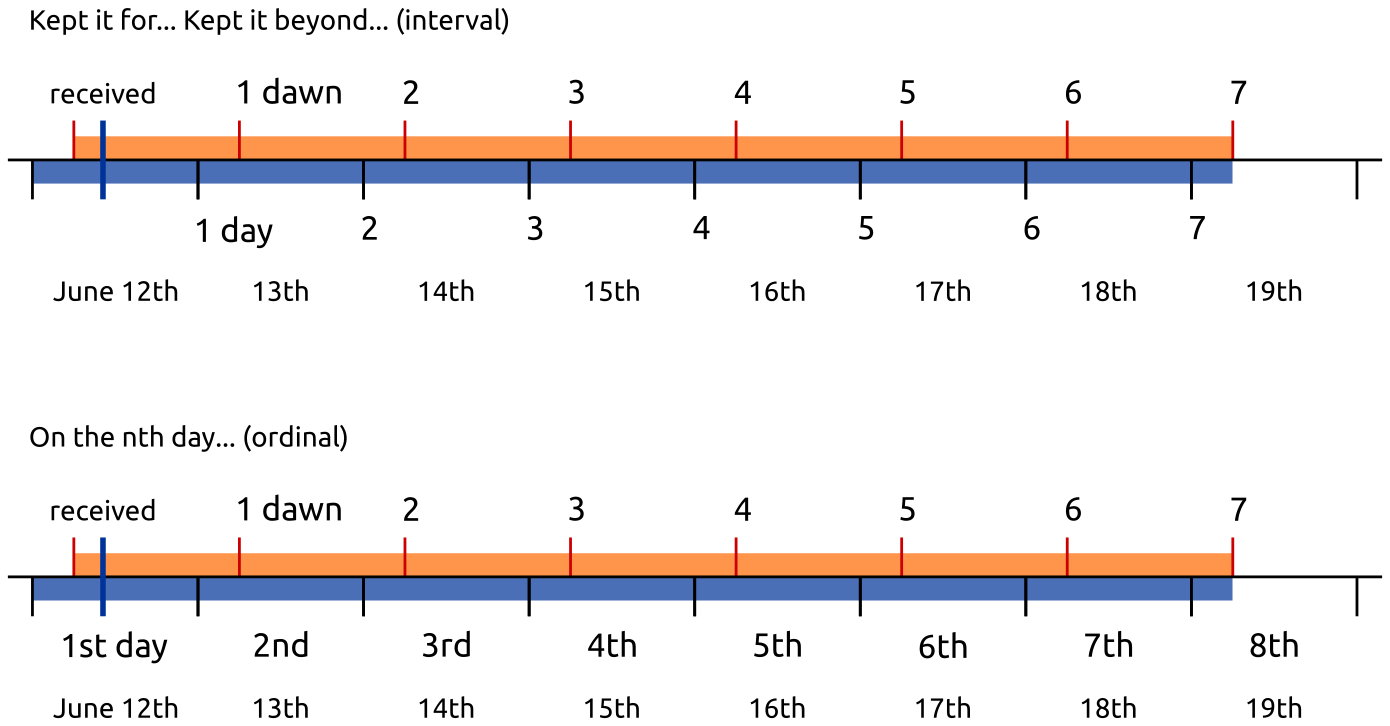
\includegraphics[width=\linewidth]{../../src/includes/figures/7-days.png}

\subsection{Breakfast tray}

After dawn, one receives a tray with bread, jams, honey, butter and
salt. At this point the lifetimes are:

\begin{itemize}
\tightlist
\item
  bread, jams: morning
\item
  honey, butter: 7 days
\item
  salt: lifetime
\end{itemize}

If the knife which one used carries bread morsels or jam into the honey
or the butter, these will be only allowable in the morning.

If one is careful to clean the knife and avoid mixing, one may use them
on the bread and keep the rest until their allowed lifetimes.

The next day, one receives a tray with only bread. One may \textbf{not}
mix the allowables from the previous day with the food received today.

Putting the salt, honey or butter (rec. yesterday) on the bread would be
Pc 38 (eating stored food).

\clearpage

\section{Pc 31, Public alms centre}

One may eat one meal at a public alms centre, not two or more days in a
row.

Origin: the group of six feel tired of almsround and keep going to the
same public kitchen.

Soup kitchens, homeless shelters, etc. Any place where all comers are
offered food free of charge.

\subsection{Non-offences}

\begin{itemize}
\tightlist
\item
  one is invited by the owners
\item
  being ill (not being able to leave)
\item
  the food is intended for bhikkhus
\item
  the centre limits the amount of food one may take (thus being able to
  censure a greedy person)
\end{itemize}

\section{Pc 32}

\section{Pc 33}

\section{Pc 34}

\section{Pc 35}

\section{Pc 36}

\section{Pc 41, Handing food to members of other religions}

One places oneself in the position of the followers of other religions.

It is not an offense to prepare food in a tray and placing it so that
they can help themselves.

\section{Pc 47, Exceeding an invitation}

When an invitation is made that one may ask for certain requisites, one
may use it until four months, unless it has been repeated, or is a
permanent invitation.

\subsection{Non-offenses}

\begin{multicols}{2}

\begin{itemize}
\tightlist
\item
  from relatives
\item
  for the sake of another
\item
  from one's own resources
\item
  being ill, if one shows consideration
\end{itemize}

\end{multicols}

``The time period for which we were invited has passed, but we have need
of medicine.''


\chapter{Money}

\begin{itemize}
\tightlist
\item
  \textbf{NP 10,} Fund with steward
\item
  \textbf{NP 18,} Gold, silver and money
\item
  \textbf{NP 19,} Selling or buying
\item
  \textbf{NP 20,} Trade
\end{itemize}

\section{NP 10, Fund with steward}

``For anyone for whom gold and silver are allowable, the five strings of
sensuality are also allowable. {[}\ldots{]} That you can unequivocally
recognize as not the quality of a contemplative, not the quality of one
of the Sakyan sons.''
(\href{https://www.dhammatalks.org/suttas/SN/SN42_10.html}{SN 42.10})

The purpose of the rule is to free bhikkhus from the complex
responsibilities of buying and selling, while facilitating the means and
protocols for their support with money.

Origin: Mendaka offers funds for the Sangha.

A bhikkhu is not allowed to accept other funds either, such as jewels,
commodities, land, livestock, etc.

A bhikkhu may designate a lay steward to manage funds offered for the
bhikkhu's support.

If the bhikkhu harasses the steward with impatient prompting, even if he
obtains the requisite, the item must be forfeited and the NP offense
confessed.

If the bhikkhu exceeds the number of allowed promptings, he incurs the
NP offense when obtaining the item.

A verbal prompting may be substituted with two silent ones: from 6
verbal and 0 silent, to 0 verbal and 12 silent.

If the steward fails to use the funds to support the bhikkhu, he should
inform the donors.

When speaking with the steward, the bhikkhu should indicate what he
needs, but may not use commands to tell them, `Give me an X, get an X
for me with the fund'.

Funds for the Sangha or a group follow the same protocols.

Funds set up for one kind of \emph{lahubhaṇḍa} may be used for another
kind, with a decision via \emph{apalokana-kamma}.

Funds set up for \emph{garubhaṇḍa} (lodgings, furniture, etc.) may not
be diverted for \emph{lahubhaṇḍa}, but NP 20 allows the community to
arrange \emph{garubhaṇḍa} to be sold and purchase \emph{lahubhaṇḍa}.

Examples: paying for electricity from the `cat's fund' (\emph{lahubh.}
to \emph{lahubh.}), selling land to buy another (\emph{garubh.} to
\emph{garubh.}).

Restricted funds may only be used for the designated purpose (Trust
law). Example: donation form selection options.

In the case of invitations, follow the four-month period protocol in Pc
47.

There is no exemption for relatives or people who have invited the
bhikkhu to ask.

\textbf{Object:} A fund left with a steward to buy robe cloth, or any
fund for any type of requisite (including construction or book
printing).

\enlargethispage*{\baselineskip}

\textbf{Steward:} a layperson or entity responsible for handling funds
or transactions on behalf of a bhikkhu or group of bhikkhus.

Three types of stewards:

\begin{itemize}
\tightlist
\item
  Indicated by the bhikkhu

  \begin{itemize}
  \tightlist
  \item
    The bhikkhu points the person out
  \item
    The donor gives funds to the steward and tells the bhikkhu
  \end{itemize}
\item
  Indicated by the donor or messenger

  \begin{itemize}
  \tightlist
  \item
    The donor or messenger chooses the steward and tells the bhikkhu
  \end{itemize}
\item
  Indicated by neither

  \begin{itemize}
  \tightlist
  \item
    Someone overhears the conversation and volunteers to act as steward
  \item
    The donor gives funds to the steward, but doesn't tell the bhikkhu
  \end{itemize}
\end{itemize}

\textbf{Given unknowingly, without consent:} One may determine ahead of
time (e.g. right now), ``If at any time in the future I am given money
without me being aware of it, I am not consenting to it as received and
accepted for my sake.''

\subsection{Protocol for accepting funds}

Allowable:

If you are asked who the steward is and you point out a layperson and
say, ``That person is the steward''.

Unallowable:

\begin{itemize}
\tightlist
\item
  Accepting money (see NP 18). You should tell the donor that bhikkhus
  don't accept money.
\item
  If a donor asks you who your steward is and you say, ``Give it to
  him'' or ``He will keep it'' (see NP 18).
\item
  If a donor asks you who your steward is and you say, ``He will buy
  it'' or ``He will get it in exchange'' (see NP 20).
\item
  If the donor asks, ``Who should I give this to?'' and you point
  someone out. A wise policy instead is to broach the topic of stewards
  so that the donor asks a question to which you may give an allowable
  answer.
\end{itemize}

\section{NP 18, Gold, silver and money}

A bhikkhu is forbidden to accept gifts of money, getting others to
accept them, or consent to it being placed next to him.

\emph{Perception} is not a mitigating factor.

\emph{Intention} is not a mitigating factor. The bhikkhu may not accept
the money for someone else's sake.

NP offense: the money is forfeit, can not be used for the benefit of
bhikkhus.

\emph{Discussion:} unaware of receiving money (wrapped in a bolt of
cloth, hidden with food offerings).

When informing lay supporters who wish to make a donation, the proper
language should be used, i.e.~not giving them instruction what to do
with their money.

If the donor does not intend the money for the bhikkhu (i.e.~offering it
to support the monastery in general), it is not an offense to allow them
to place the money next to the bhikkhu.

If someone drops money into a bhikkhu's bowl against his protest, he may
ask someone to remove it without an offense. The offense is incurred
when he start walking away with it.

The term `gold or silver' includes the materials, and whatever is used
as currency.

\clearpage

A currency is:

\begin{itemize}
\tightlist
\item
  used for the purpose of general exchange
\item
  have a standardized value
\item
  presentable by any bearer
\end{itemize}

Not a currency:

\begin{itemize}
\tightlist
\item
  a money order or check made out to a specific person
\item
  credit- and debit cards
\item
  a store's voucher, gift card, or discount points
\item
  food stamps
\item
  promissory notes
\end{itemize}

Credit cards are not a currency, but are not allowable to use (see NP
20).

\emph{Inheritance:} The executor holds the money before distributing it
to the beneficiaries. The bhikkhu may advise the executor to put the
money into a certain Trust.

A bhikkhu may own property, land (not for agriculture), houses, etc. but
not the money to manage it.

In some monasteries two Trusts are setup, where one may only own land
and property, and the other may only hold money.

\emph{Store credit:} a lay person may leave money at a store, and
arrange that they serve a bhikkhu using that credit when he asks (Amazon
voucher, restaurant, pastry shop).

\subsection{Non-offenses}

There is no offense for a bhikkhu, in the monastery, to pick up gold or
money and put it away for safe keeping.

\section{NP 19, Selling or buying}

This covers the case when a bhikkhu would instruct someone else to
arrange the trade, without himself accepting the money.

There is no allowance for `wording things right'
(\emph{kappiya-vohāra}).

A bhikkhu may advise a steward to sell some items and purchase others,
but \textbf{may not} instruct them to sell something or invest money for
profit. A bhikkhu may give instruction to order things for the
monastery.

\section{NP 20, Trade}

Exchange of items with lay people or members of other sects.

Giving gifts to lay people at a meal invitation is a way of corrupting
families (bhikkhus of the group of six were giving flowers, etc. to
supporters).

\emph{Origin:} Ven. Upananda exchanges a nicely made robe for a cloak
with a wanderer, who later regrets the trade and wants it back.

Credit cards or checks don't count as currency, but any trade arranged
with them would come under this rule.

\enlargethispage*{\baselineskip}

\subsection{Non-offenses}

\begin{itemize}
\tightlist
\item
  asking for the price
\item
  informing the steward or seller (e.g.~``I have this. I need X'') and
  letting the steward or seller arrange the exchange
\item
  if the other person is a bhikkhu or novice
\item
  saying, ``Give X for Y'' when engaging in trade with your parents
\item
  telling the steward, ``Don't take it'' when you think the steward is
  getting a bad deal
\end{itemize}


\chapter{14. Arguments 1}
\renewcommand*{\theChapterTitle}{14. Arguments 1}

\section*{Discussion}

% \subsection*{Sg 10, Schismatic group}

The Buddha made many efforts to end the quarrel at Kosambi which was heading to
a schism but in the end concluded: “These foolish men are as though infatuated;
it is not easy to persuade them,” rising up from his seat, departed. How did the
issue get resolved?

\bigskip

% A: The lay people, upset that the monks of Kosambi drove the Buddha away,
% stopped respecting the monks and offering them alms food, thinking it might
% help to resolve the issue. The monks of Kosambi, as a result, sort out the
% Buddha to resolve this vinaya question.

% \subsection*{Sg 11, Supporting a schismatic group}

Why is this rule of a monk with one, two or three supporters only?

\bigskip

% Four is already a split group

% \subsection*{Sg 12, Not accepting admonishment}

If a bhikkhu difficult to admonished persist with his behaviour, and is then
formally rebuked by the sangha in a sanghakamma of one motion and three
announcements – can he be made to carry out the sanghadisesa penalty?

\bigskip

What additional procedure should the community to carry out?

\bigskip

% A Community planning to impose any of these rules on one of its members should
% be prepared to recite the transaction statement for suspension against him as
% well, in the case that he is so stubborn that he will not see his fault or
% admit his sanghadisesa.

% \subsection*{Sg 13, Not accepting a rebuke or banishment}

What are some examples of wrong modes of livelihood (for bhikkhus) which can lead to corrosion of families?

\bigskip

% \begin{itemize}
% 
% \item running messages and errands - participating in political campaigns.
% 
% \item scheming, talking, hinting, belittling others for the sake of material
%   gain, pursuing gain with gain – giving hoping to receive more
% 
% \item Practicing worldly arts, e.g., medicine, fortune telling, astrology,
%   exorcism, reciting charms, casting spells, performing ceremonies to counteract
%   the influence of the stars, determining propitious sites, setting auspicious
%   dates (for weddings, etc.), interpreting oracles, auguries, or dreams.
% 
% \end{itemize}

% \subsection*{Pc 9, Telling an unordained person about serious offence}

What is meant by serious offence?

\bigskip

There is a non-offense if one tells a lay person the action of an ofference if
one does not mention the class, or the class, if one does not mention the action
– how can this be a problem?

\bigskip

% Lay people generally know about the rules these days.

When might it be helpful to make use of this rule?

\bigskip

% a) A bhikkhu commits a serious offence and refuses to acknowledge it.
%
% b) Assuming to be a bhikkhu after doing a parajika or refusing to do
% rehabilitations after sanghadisesa – the sangha could then authorize a bhikkhu
% to inform the lay community – the bhikkhus supporters – to exert pressure on
% him to submit to the penalty.
%
% c) It could be used to help a weak-willed bhikkhu in mending his ways.

% \subsection*{Pc 12, Evasive reply}

What is meant by evasive or uncooperative? 

\bigskip

% Evasive – one leads the talk aside
% 
% Uncooperative – one remains silent

What are the allowable reasons for remaining silent, asking questions, not speaking to the point?

\bigskip

% Not understanding what is being said, too ill to speak, feeling that to speak
% will create conflict or dissension in the Community, feeling that the Community
% will carry out a transaction unfairly or not in accordance with the rule.

% \subsection*{Pc 13, Criticising community official}

Would there be an offense to criticize and complain about to others, a bhikkhu
who is not a community official?

\bigskip

% dukkata 

To criticize a biased community official to his face to hurt his feelings?

\bigskip

% Pc2 regardless of whether his behaviour has been biased or not.

A bhikkhu complains that the lodgings monk gives the best dwellings to his friends – any offense?

\bigskip

% No offense if the official acts from the four causes of bias – desire, aversion,
% delusion, fear. Why is there no offense?

% A qualifying factor for a community official is that he is unbiased.


\chapter{Arguments 2}

\begin{itemize}
\tightlist
\item
  \textbf{Pc 54,} Disrespectful after admonition
\item
  \textbf{Pc 64,} Concealing another's serious offence
\item
  \textbf{Pc 65,} Ordaining someone less than 20 years old
\item
  \textbf{Pc 68,} Not relinquishing an evil view
\item
  \textbf{Pc 69,} Suspended bhikkhu
\item
  \textbf{Pc 70,} Expelled novice
\item
  \textbf{Pc 74,} Hitting a bhikkhu
\item
  \textbf{Pc 75,} Threatening gesture
\end{itemize}

\section{Pc 54, Disrespectful after admonition}

Different offences for showing disrespect:

When the admonition is related to a specific rule in the Vinaya, the
offence is \emph{pācittiya}.

When the admonition relates to general behaviour of being self-effacing,
scrupolous, etc., the offence is \emph{dukkaṭa}.

The validity of the admonition is not a factor.

Disrespect can be expressed to the rule, to the person, by word or by
gesture.

There is no offence in politely discussing that one was taught
differently somewhere else.

A ploy to avoid being criticized is \emph{Pc 71}.

\section{Pc 64, Concealing another's serious offence}

A bhikkhu doesn't inform the community about another bhikkhu's serious
offence, possibly out wishing to save him from the consequences or
embarrassment.

There is no offence in not informing the community, if one's motivation
is not to hide the offence, but for example waiting to inform the abbot
first.

\section{Pc 65, Ordaining someone less than 20 years old}

A person's age here is counted from the time he had become a fetus in
her mother's womb (add six months to the date of birth).

\section{Pc 68, Not relinquishing an evil view}

A bhikkhu wants to do something he knows to be declared improper for
him:

\begin{quote}
``As I understand the Dhamma taught by the Blessed One, those acts the
Blessed One says are obstructive, when engaged in are not genuine
obstructions.''
\end{quote}

`Obstructions' include the five \emph{ānantarika-kamma}, persisting in
extreme wrong views and intentional transgression of training rules.

\enlargethispage*{\baselineskip}

The other bhikkhus should reprimand him. If he relinquishes his view,
there is no penalty.

A bhikkhu who doesn't respond after being formally rebuked, should be
suspended.

\clearpage

\section{Pc 69, Suspended bhikkhu}

Other bhikkhus should not commune, affiliate or lie down in the same
dwelling with a suspended bhikkhu.

There is no offence if one knows the bhikkhu has already given up his
wrong view, but has not yet been formally restored.

\section{Pc 70, Expelled novice}

A novice who persists in holding onto such wrong views should be
expelled. A novice may be also expelled when he breaks his precepts
habitually and is not intending to correct his behaviour.

Afterwards, the bhikkhus should not befriend him, receive his services,
commune or lie down with him in the same dwelling.

\section{Pc 74, Hitting a bhikkhu}

Hitting a bhikkhu in anger is a \emph{pācittiya}, an unordained person
is a \emph{dukkaṭa} offence.

It is not a factor whether the other person is hurt or not.

It is not an offence to hit another person when being in physical danger
and wanting to escape.

\section{Pc 75, Threatening gesture}

Raising the palms or making some other threatening gesture out of anger.


\chapter{Arguments 3}

\begin{itemize}
\tightlist
\item
  \textbf{Pc 77,} Provoking anxiety
\item
  \textbf{Pc 78,} Eavesdropping in an argument
\item
  \textbf{Pc 63,} Reopen a closed issue
\item
  \textbf{Pc 79,} Complaining about a community decision
\item
  \textbf{Pc 80,} Leaving a community meeting
\item
  \textbf{Pc 81,} Complaining about favouritism
\end{itemize}

\section{Pc 77, Provoking anxiety}

Telling a bhikkhu that he might have broken a rule, or otherwise
deliberately provoking his anxiety, thinking, `This way, even for just a
moment, he will have no peace.'

\emph{Result} is a factor, the bhikkhu has to experience anxiety even
for a moment.

There is no offense in discussing offenses out of genuine concern, or
for the sake of clarifying the training.

\section{Pc 78, Eavesdropping}

Deliberately listening in while others are in argument or other
discussion, only for the sake of using what they say against them, even
if only for making them feel embarrassed.

Reading a bhikkhu's private documents (papers, files, emails) also
fulfils \textbf{Effort}.

When one has business to do where some others are debating an issue, one
should cough or otherwise signal being present.

\section{Pc 63, Reopen a closed issue}

Relevant issues may be disputes, accusations, offenses, or relating to
duties.

The purpose of the rule is to avoid burdening and encumbering a
community, only to satisfy one bhikkhu's personal agenda.

Once an issue has been discussed and dealt with properly, agitating to
re-open it fulfils \textbf{Effort}: `They are inexperienced and dealt
with it poorly. That's not the way to do it.'

\textbf{Intention:} one knows that the issue was dealt with properly
(but perhaps is not content to follow the agreement).

The rule applies to decisions in the past, or when one was not present
at the meeting. One implicitly agrees to such established decisions by
asking to live at a monastery, expressed by asking for dependence
(\emph{nissaya}) and other protocols.

\subsection{Non-offenses}

\begin{itemize}
\tightlist
\item
  Re-opening an issue when it was in fact not dealt with properly

  \begin{itemize}
  \tightlist
  \item
    not in accordance with the rules, decision by an incomplete group,
    unjustified penalties, etc.
  \end{itemize}
\item
  New matters arising out of old decisions are new issues
\end{itemize}

\section{Pc 79, Complaining about a community decision}

\emph{Origin:} Some group-of-six bhikkhus don't want to go to a meeting
and send their consent (\emph{chanda}). The bhikkhus use the opportunity
to make a decision against them. The group-of-six bhikkhus complain that
they wouldn't have consented to \emph{that}.

Community transactions have to be carried out with all the bhikkhus
present, who are currently within the monastery area. The Pāṭimokkha
recitation at the \emph{uposatha-kamma} is one example.

There is allowance for one to be absent (such as when being too sick) by
sending one's consent (\emph{chanda}) to whatever decisions are made at
the meeting.

A valid transaction has to be carried out by a complete assembly, in
order to prevent small factions making independent decisions.

``All the bhikkhus of common affiliation within the territory are either
present at the meeting (sitting within \emph{hatthapāsa}) or have given
their consent by proxy, and no one -- in the course of the transaction
-- makes a valid protest against its being carried out.'' (Mv.IX.3.5-6)

\subsection{Non-offenses}

\begin{itemize}
\tightlist
\item
  the decision was not in accordance with the rule
\item
  incomplete assembly
\item
  unjustified penalties
\end{itemize}

\section{Pc 80, Leaving a community meeting}

\emph{Origin:} one group-of-six bhikkhu leaves a meeting in order to
prevent a transaction being carried out against him.

In order for the transaction relating to a bhikkhu be valid, has to be
either present or given his consent.

\textbf{Effort:} he goes beyond \emph{hatthapāsa} of the bhikkhus in the
meeting without first giving his consent.

There is no offense if one leaves the meeting for a different purpose,
such as being ill, can't wait to use the toilet, or thinking `I'll be
right back.'

Nonetheless, it is better to give one's consent before leaving the
meeting.

\section{Pc 81, Complaining about favouritism}

The community is not allowed to transfer the ownership of
\emph{garubhaṇḍa} articles (land, dwelling, furniture, expensive tools,
etc.) to individual bhikkhus.

Light or inexpensive (\emph{lahubhaṇḍa}) articles may be given to an
individual with the proper procedure.

There may be a formal meeting and community transaction, or an informal
meeting where the community members may object.

Complaining after one \emph{has not} objected to the article being given
to an individual, fulfils \textbf{Effort}.

There is no offense to complain out of valid concerns (as in \emph{Pc
13}, criticizing a community official), such as habitual favouritism,
anger, delusion or fear, which means the transaction was invalid.


\chapter{17. Dwellings}
\renewcommand*{\theChapterTitle}{17. Dwellings}

\section*{Discussion}

% \subsection*{Sg 6, Too large hut without sponsor or approval}

A bhikkhu, by means of begging, is building a kuti for himself, without a
sponsor. What are the two factors could then lead to a sanghadisesa offense?
When is this offense incurred?

\begin{solution}
  He does not get bhikkhus to approve the site and carry out a sanghakamma, the
  kuti is more than 3m long externally or 1.75m wide internally. The offense is
  incurred when the kuti is finished.
\end{solution}

\bigskip

% Sg 7 Large hut without approval

What are the differences here between Sg 6 and Sg 7?

\begin{solution}
  In Sg 7 it is a large dwelling and no lower or upper limits to the size.

  He has a sponsor for the project – it is not built through begging. 
\end{solution}

\bigskip

% Pc 14 Leaving bed or bench

What is the distance at which it is considered you have departed from the furnishings?

\begin{solution}
  One leḍḍupāta -- 18 meters.
\end{solution}

\bigskip

A bhikkhu departs from his mattress set out to air in the sun, intending to
return immediately, does he incur an offense?

\begin{solution}
  No - there is no offense if one departs having set furnishings belonging to
  the Community or another individual out in the sun with the purpose of drying
  them, and thinking, “I will put them away when I come back.”

  Point from Vinaya-mukha: “This training rule was formulated to prevent
  negligence and to teach one to care for things. It should be taken as a
  general model.”
\end{solution}

\bigskip

If there is to be an open-air meeting, who is responsible for the seats set out
in the open?

\begin{solution}
  The host bhikkhus are responsible for any seats set out in the open, until the
  visiting bhikkhus claim their places, from which point the visitors are
  responsible.
\end{solution}

\bigskip

Would the open yet roofed area on our kuti’s count as out in the open under Pc 14 (leaving bed or bench)?

\begin{solution}
  Unlikely, as it should be a fully open area.
\end{solution}

\bigskip

% Pc 15 Spread bedding

Suggest some practical reasons for Pc 15 (spread bedding).

\begin{solution}
  Origin story: the purpose of the rule is to prevent the bedding’s being left
  so long in an unoccupied dwelling that it attracts ants, termites, or other
  pests.

  Vinaya-mukha: leaving bedding and other belongings scattered about in a
  dwelling might inconvenience the resident bhikkhus in that they could not
  easily allot the dwelling to another bhikkhu.
\end{solution}

\bigskip

% Pc 16 * Intruding on bhikkhu’s sleeping place

How is the bhikkhu who should not be forced to be moved defined in the Vibhanga?

\begin{solution}
  Knowing the dwelling’s current occupant is a senior bhikkhu, a sick one, or
  one to whom the Community (or its official) has assigned the dwelling.
\end{solution}

\bigskip

Suggest valid reasons for intruding on a bhikkhu’s dwelling.

\begin{solution}
  Illness, suffering from cold or heat, dangers outside.
\end{solution}

\bigskip

% Pc 17 Causing a bhikkhu to be evicted

Does Pc 17 (causing a bhikkhu to be evicted) cover physical evication (throwiong someone out) and verbal
eviction (ordering someone to leave) in the same way?

\begin{solution}
  Yes the offense is the same for both.
\end{solution}

\bigskip

Suggest some valid reasons for evicting someone.

\begin{solution}
  Insane, unconscientious in their behaviour, a maker of quarrels, strife,
  dissension in the community. A teacher may evict their student or his
  belongings from his dwelling if he is not properly observing his duties.
\end{solution}

\bigskip

% Pc 18 Bed on an unplanked loft

What is the purpose of Pc 18 (bed on an unplanked loft), as indicated in the origin story?

\begin{solution}
  To guard against injury to a bhikkhu living under the loft: He might get hit
  on the head if any of the detachable legs fall down through the joists of the
  loft – therefore no offense of the space under the loft is not suitable as a
  dwelling or if there is no one underneath.
\end{solution}

\bigskip

% Pc 19 Supervising the building work

What can be understood as the reason for Pc 19 (supervising the building work)?

\begin{solution}
  The non-offense clauses show clearly that the rule is aimed at preventing
  bhikkhus from abusing the generosity of the person sponsoring the building
  work.
\end{solution}

\bigskip

% Pc 87 Tall bed or bench

Suggest the main purpose for Pc 87 (tall bed or bench).

\begin{solution}
  The purpose of this rule is to prevent bhikkhus from making and using
  furnishings that are high and imposing.
\end{solution}

\bigskip

Describe what the factors of effort and intention make under Pc 87.

\begin{solution}
  Effort: One acquires it after making it or having it made. Intention: for
  one’s own use.
\end{solution}

\bigskip

What can be done if one receives from another an oversize bed or bench.

\begin{solution}
  One can cup down the legs the regulation size before use.
\end{solution}

\bigskip

You are visiting a lay friend, and they invite you to make use of a high bed,
with long legs, is it suitable to use it, what would be a suitable course of
action?

\begin{solution}
  Cv.VI.8 allows that if furnishings of the sort unallowable for bhikkhus to own
  themselves are in a lay person’s house (and belong to the lay person, says the
  Sub-commentary) bhikkhus may sit on them but not lie down on them.
\end{solution}

\bigskip

What to do if not using the bed would seriously offend the lay supporter?

% Pc 88 Cotton stuffing

What is the purpose of Pc 88 (cotton stuffing)? 

\begin{solution}
  The purpose of all this is to keep bhikkhus from using furnishings that are
  extravagant and ostentatious.
\end{solution}

\bigskip

What comments from the Vinaya-mukha give guidance on how to use Pc 88 – how
can this apply in the monastery and when visiting a lay persons home?

\begin{solution}
  Vinaya-mukha mentions, though, standards of what counts as extravagant and
  ostentatious vary from age to age and culture to culture (Some of the things
  allowed in the Canon and commentaries now seem exotic and luxurious; and other
  things forbidden by them, common and ordinary.)

  Thus the wise policy, in a monastery, would be to use only those furnishings
  allowed by the rules and regarded as unostentatious at present. When visiting
  a lay person’s home, to avoid sitting on furnishings that seem unusually
  grand.
\end{solution}

\bigskip

A bhikkhu makes arranges for his residence for the Vassa at the house of three different lay supporters. He spends one month at each residence.

Is this a suitable arrangement for him?

Does this break his determination made at the beginning of the Vassa?

What would be the minimum procedure he should carry out at each residence?

\bigskip

A bhikkhu wishes to spend the Vassa outside in a tent, but still within the monastery \emph{sīma}.

What would be required to make this a suitable Vassa residence for him?

\begin{solution}
  During the Vassa one needs to be in an accommodation that has a door that can
  be `opened and closed' (see BMC 2, chapter Rains-residence).

  A tent doesn't fall under this definition, but if the bhikkhu is allocated an
  accommodation in the monastery with a proper door, which he has access to any
  time, he may spend the days and nights somewhere else, if it is still within
  the \emph{sīma}.

  The community may discuss the possible locations of the tent, in order for the
  bhikkhu not be disturbed by lay visitors or country-walkers passing by.

  One may also determine a \emph{sattaha} and go for a short tudong, camping
  outside the \emph{sīma}, if the conditions are suitable.
\end{solution}

\chapter{18. Bowls}
\renewcommand*{\theChapterTitle}{18. Bowls}

\section*{Discussion}

% \subsection*{NP 21, Keeping extra bowl}

You would like to make use of a smaller bowl for a tudong – is there a way of
doing this without fully relinquishing your current bowl?

\begin{solution}
  Make use of shared ownership.
\end{solution}

  \bigskip

% \subsection*{NP 22, Asking for new bowl}

A bhikkhu asks for a new bowl, even though his current bowl is not broken.
Following the protocol he relinquishes his new bowl to the sangha. In what way
might he receive it back?

\begin{solution}
  If none of the Bhikkhus exchange the new bowl for theirs, the offending
  monk will receive the bowl once the last monk is reached.
\end{solution}

\bigskip

% \subsection*{Pc 60, Hiding another's requisites}

Is there an offense in putting away a needle case that a monk has left laying around? 

\begin{solution}
  Putting away properly is no offense.
\end{solution}

\bigskip

You hide your friend's robe, knowing he will find it funny too – is ther an offense?

\bigskip

\begin{solution}
  Friendly or malicious – offense all the same.
\end{solution}

% \subsection*{Pc 86, Needle box}

If one obtains a bone, ivory, or horn needle box made by another—not at one’s instigation—offense?

\begin{solution}
  Using it entails a dukkata. 
\end{solution}

\bigskip

A bhikkhu finds a large bone while walking and carves it into a needle box as a gift – any offense?

\begin{solution}
  Dukkata
\end{solution}

\bigskip

What if he carves a robe- or belt fastener instead?

\begin{solution}
  No – these are allowable in the non-offense clause. 
\end{solution}

\bigskip

What is the general principle derived from Pc 86 (Needle box)?

\begin{solution}
  The Buddha formulated this rule to put a stop of a ‘bhikkhu fad’ – where a
  certain requisite becomes fashionable to the point of putting pressures on a
  inconveniencing donors.
\end{solution}


\chapter{Women 2}

\begin{itemize}
\tightlist
\item
  \textbf{Ay 1,} sitting privately with a woman
\item
  \textbf{Ay 2,} sitting out of earshot with a woman
\item
  \textbf{Bhikkhunīs,} summary of related rules: NP 4-5, NP 17, Pc
  21-30, Pd 1-2.
\end{itemize}

\section{Ay 1, sitting privately with a woman}

The \emph{aniyata} (indefinite) rules highlight two difficult situations
and require the community to examine them, instead of assigning a
definite offense.

\emph{Origin:} Lady Visākhā sees the Ven. Udāyin sitting at a concealed
place with a girl who is newly married.

\begin{quote}
`It is unfitting, venerable sir, and improper, for the master to sit in
private, alone with a woman {[}\ldots{]} Even though the master may not
be aiming at that act, cynical people are hard to convince.'
\end{quote}

A \emph{woman} here means a female human being, `even one born that very
day, all the more an older one.'

\emph{Sitting:} The situation includes lying down.

\emph{Private:} Private to the eye and ear, \emph{and} concealed. No one
else can see their facial expressions or hear what they say.

\emph{A secluded seat:} concealed behind a wall, a closed door, a large
bush. Sufficient cover for sexual activity.

This is already an offense under \emph{Pc 44 (secluded seat)}, but this
rule also covers the heavier offenses.

The bhikkhu community should investigate, hearing out the relevant
individuals, and deciding on imposing the penalty or not.

They may deal with the bhikkhu only in terms of what he admits having
done. They may cross-question him as a group, until they are satisfied
that he is telling the truth.

The decision must be unanimous, and the bhikkhu in question must accept
that his action was an offense. Otherwise the case has to be left
unsettled.

\section{Ay 2, sitting out of earshot with a woman}

\emph{Origin:} Lady Visākhā sees the Ven. Udāyin sitting again with that
girl, private to the eye and ear but this time \emph{not} concealed.

A \emph{woman} here means one who can recognize lewd remarks.

\clearpage

\section{Bhikkhunīs}

\textbf{NP 4:} Having an unrelated bhikkhunī wash, dye, or beat a used
robe.

\textbf{NP 17:} Same with wool. The group of six are harassing the
bhikkhunīs.

\textbf{NP 5:} Accepting robe-cloth from an unrelated bhikkhunī by hand,
without giving anything in exchange.

\textbf{Pc 21:} Unauthorized exhortation to bhikkhunīs.

\textbf{Pc 22:} Authorized exhortation, but after sunset.

\textbf{Pc 23:} Exhortation at the bhikkhunīs' quarters.

\textbf{Pc 24:} Accusing to exhort bhikkhunīs for worldly gain.

\textbf{Pc 25:} Giving robe-cloth to an unrelated bhikkhunī without
exchange.

\textbf{Pc 26:} Sewing robe-cloth for an unrelated bhikkhunī.

\textbf{Pc 27:} Travelling by arrangement with a bhikkhunī.

\textbf{Pc 28:} A boat trip by arrangement with a bhikkhunī.

\textbf{Pc 29:} Eating alms-food prompted by a bhikkhunī to be given.

\textbf{Pc 30:} Sitting in private and alone with a bhikkhunī.

\textbf{Pd 1:} Receiving and eating alms-food from an unrelated
bhikkhunī in a village.

\textbf{Pd 2:} Letting a bhikkhunī standing where the bhikkhus are
eating, as though giving instructions on which bhikkhu should receive
what.

\emph{NOTE:} A bhikkhu and a sīladhārā should not give personal gifts to
one another, or use a messenger to send the gift, even if it is in
exchange. The bhikkhu community as a whole may decide to offer items to
a sīladhārā, or the sīladhārā community as a whole may decide to offer
items to a bhikkhu.


\chapter{20.A. Misc 2}
\renewcommand*{\theChapterTitle}{20.A. Misc 2}

\begin{exam}{\autoExamName}

  \begin{problem*}

    Are there offences?

    \begin{parts}

      \item An old battleship, still in the harbour, is used as a museum. Lay
      friends invite the bhikkhu to visit it together, who agrees to go.

      \bigskip

      \begin{answers}{3}
        \bChoices
        \Ans0 pācittiya\eAns
        \Ans1 dukkaṭa\eAns
        \Ans0 no offences\eAns
        \eChoices
      \end{answers}

      \begin{solution}
        Dukkata as a derived offence of Pc 48 (watching battle).

        Dukkata as not a proper place for a bhikkhu to be, `a wrong resort'.

        Similar situation is walking past the residence of the president, which is guarded by the military.

        A war memorial would be no offence, as it's not dedicated to war, but to those who lost (or gave) their lives in it.
      \end{solution}

      \bigskip

      \item A bhikkhu is visiting a prison inmate on his request for religious
      counselling. There are military vehicles parked in front of the prison
      building. The bhikkhu walks around them amused, taking photos.

      \bigskip

      \begin{answers}{3}
        \bChoices
        \Ans0 pācittiya\eAns
        \Ans0 dukkaṭa\eAns
        \Ans1 no offences\eAns
        \eChoices
      \end{answers}

      \begin{solution}
        Dukkata as not a proper place for a bhikkhu to be, `a wrong resort'.
      \end{solution}

      \bigskip

      \item A bhikkhu's cousin is an officer in the army. He is moved to a
      station nearby for a time, and invites the bhikkhu to a tour of the base.
      They walk around, looking at the soldiers performing their daily routine.

      \bigskip

      \begin{answers}{3}
        \bChoices
        \Ans1 pācittiya\eAns
        \Ans0 dukkaṭa\eAns
        \Ans0 no offences\eAns
        \eChoices
      \end{answers}

      \begin{solution}
        Not an offence to go, but an offence to amuse oneself there.
      \end{solution}

      \bigskip

      \item A bhikkhu finds an abandoned surf-board on the beach. He takes off his upper
      robe and takes the surf-board for a ride in the water.

      \bigskip

      \begin{answers}{3}
        \bChoices
        \Ans1 pācittiya\eAns
        \Ans0 dukkaṭa\eAns
        \Ans0 no offences\eAns
        \eChoices
      \end{answers}

      \bigskip

      \item Two bhikkhus were advised by their doctor to swim. They go down to a
      river for swimming. When they arrive, they start throwing water at each
      other for a laugh.

      \bigskip

      \begin{answers}{3}
        \bChoices
        \Ans1 pācittiya\eAns
        \Ans0 dukkaṭa\eAns
        \Ans0 no offences\eAns
        \eChoices
      \end{answers}

      \bigskip

      \item Two bhikkhus are on tudong. After sunset, they start telling each
      other ghost stories. They get so spooked that they don't dare to sleep.

      \bigskip

      \begin{answers}{3}
        \bChoices
        \Ans0 pācittiya\eAns
        \Ans0 dukkaṭa\eAns
        \Ans1 no offences\eAns
        \eChoices
      \end{answers}

      \begin{solution}
        Pācittiya if done for the excitement of scaring each other.

        No offence if this is not the reason, and they just remember ghost stories.
      \end{solution}

      \bigskip

      \item A bhikkhu waits behind a corner, and suddenly steps forward when he
      hears a bhikkhu coming. He seems very amused with the startled expression
      on his face.

      \bigskip

      \begin{answers}{3}
        \bChoices
        \Ans1 pācittiya\eAns
        \Ans0 dukkaṭa\eAns
        \Ans0 no offences\eAns
        \eChoices
      \end{answers}

    \end{parts}

  \end{problem*}

\end{exam}

\chapter{20.B. Misc 2}
\renewcommand*{\theChapterTitle}{20.B. Misc 2}

\chapter{21. Sekhiyas 1}
\renewcommand*{\theChapterTitle}{21. Sekhiyas 1}

\begin{exam}{\autoExamName}

  \begin{problem*}
    \textbf{Do} or do \textbf{Not}?

    \bigskip

    \begin{parts}

    \item \TF{D} Walking on the street with a big sun hat on hot day.

    \bigskip

    \item \TF{N} Sitting in an angsa while travelling in a car.

    \bigskip

    \item \TF{D} Visiting the town hall, wearing the upper-robes on both shoulders.

    \bigskip

    \item \TF{N} Walking along a crowded beach in an angsa.

    \bigskip

    \item \TF{N} Sitting in an angsa in a public park.

    \bigskip

    \item \TF{N} Using a corn-field as cover for defecating.

    \bigskip

    \item \TF{N} Walking on the street, explaining a story and wildly gesticulating with the arms for emphasis.

    \bigskip

    \item \TF{D} Walking along a river, stopping to urinate, away from the river.

    \bigskip

    \item \TF{N} Being in a hurry before the \emph{uposatha-kamma}, pulling up the upper robe and urinating.

    \bigskip

    \item \TF{N} Wearing a hat inside a supermarket.

    \bigskip

    \item \TF{N} Having parked and walked away from the car, yelling back to the driver to bring a water bottle.

    \end{parts}

  \end{problem*}

\end{exam}

\chapter{22.A. Excuses}
\renewcommand*{\theChapterTitle}{22.A. Excuses}

\begin{exam}{\autoExamName}

  \begin{problem*}

    Are there offences?

    \begin{parts}

      \item The abbot tells a bhikkhu to keep his robes within \emph{hatthapāsa}
      at dawn, strapping them to his body if necessary. The bhikkhu responds
      that this is silly, and he prefers his previous teacher's interpretation
      of `robe boundary'. He keeps his robes in the \emph{dāna-sāla} instead.

      \bigskip

      \begin{answers}{3}
        \bChoices
        \Ans1 pācittiya\eAns
        \Ans0 dukkaṭa\eAns
        \Ans0 no offences\eAns
        \eChoices
      \end{answers}

      \begin{solution}
        Pācittiya since the motive is being irritated, not wanting to bother
        with a strict interpretation of the training rule.
      \end{solution}

      \bigskip

      \item A bhikkhu is eating in a very disciplined manner when the abbot is
      around, but as soon as the abbot walks out, his manner becomes
      unrestrained, and starts chatting with his mouth full. A one-Vassa bhikkhu
      comments on this, and he responds, `Oh, you know everything now?'

      \bigskip

      \begin{answers}{3}
        \bChoices
        \Ans1 pācittiya\eAns
        \Ans0 dukkaṭa\eAns
        \Ans0 no offences\eAns
        \eChoices
      \end{answers}

      \bigskip

      \item A bhikkhu who is in charge of the monastery office, removes the list
      of Sangha regulations from the wall, hoping that the other bhikkhus will
      forget them. He spreads comments that the old \emph{kor-wat} doesn't apply now.

      \bigskip

      \begin{answers}{3}
        \bChoices
        \Ans0 pācittiya\eAns
        \Ans1 dukkaṭa\eAns
        \Ans0 no offences\eAns
        \eChoices
      \end{answers}

      \begin{solution}
        Dukkata as a derived offence, since \emph{kor-wat} rules are not those laid down by the Buddha.
      \end{solution}

      \bigskip

      \item A sāmaṇera is in charge of preparing the community breakfast. He
      always makes sure to arrange his favourite jam on the sāmaṇeras' tray.
      After he receives \emph{upasampadā}, during breakfast he sneaks the jam
      from the sāmaṇeras' tray to the bhikkhus'. When he is caught by a bhikkhu,
      he says that he is new, and nobody told him about that rule.

      \bigskip

      \begin{answers}{3}
        \bChoices
        \Ans1 pācittiya\eAns
        \Ans1 dukkaṭa\eAns
        \Ans0 no offences\eAns
        \eChoices
      \end{answers}

      \begin{solution}
        Pācittiya for taking what is not given.

        Dukkaṭa for pretending ignorance of the rule.

        One may remember that \emph{Pc 73} generously allows an excuse for not knowing the rules until the third time hearing the \emph{pāṭimokkha}, but since in their training years the anagārikas and sāmaṇeras already study the rules and participate in Vinaya classes, it is hard to believe a bhikkhu claiming genuine ignorance of not having heard of a particular training rule.
      \end{solution}

    \end{parts}

  \end{problem*}

\end{exam}

\chapter{22.B. Excuses}
\renewcommand*{\theChapterTitle}{22.B. Excuses}

\chapter{Sekhiyas 2}

\begin{itemize}
\tightlist
\item
  \textbf{Sk 27-56,} Food
\item
  \textbf{Sk 57-72,} Teaching Dhamma
\end{itemize}


\chapter{Robes 2}

\begin{itemize}
\tightlist
\item
  \textbf{NP 16,} Carrying Wool
\item
  \textbf{NP 26,} Thread
\item
  \textbf{NP 27,} Weavers
\item
  \textbf{NP 11-15,} Summary of santhatas
\end{itemize}

\section{NP 16, Carrying Wool}

One may carry the unmade wool for three yojanas
(\texttt{3*16\ =\ 48\ km}). Further than that, one should find someone
else to transport the wool for him.

If people see a bhikkhu carrying raw materials, they might assume that
he bought them, and that he is producing something to sell.

\section{NP 26, Thread}

Asking for thread and having it woven into a robe is improper protocol
for a bhikkhu.

A bhikkhu should request from his supporters what he needs, rather than
the raw materials for it.

\subsection{Non-offences}

\begin{itemize}
\tightlist
\item
  if both the supporters and weavers are his relatives
\item
  if they made invitation to ask
\item
  asking for the sake of another
\item
  by means of one's own resources
\end{itemize}

\section{NP 27, Weavers}

When his supporters are organizing requisites for a bhikkhu, such as
having a robe woven for him, he should accept what he receives. If the
supporters ask for details, he should describe what he needs to them,
instead of interfering with how they obtain it.

Origin: Ven. Upananda interferes in the process of a robe being made for
him by going to the weaver's shop and making a fuss about details.

Related to \emph{NP 8}, making stipulations about what kind of robe to
receive.

\subsection{Non-offences}

\begin{itemize}
\tightlist
\item
  the supporters are relatives
\item
  they have invited one to ask
\item
  asking for the sake of another
\item
  getting the weavers make the cloth less expensive
\item
  by means of one's own resources (e.g.~the bhikkhu hired the weavers)
\end{itemize}

\clearpage

\section{NP 11-15, Summary of santhatas}

A \emph{santhata} is a blanket or rug made of felt material. It is made
by strewing the threads over a surface, adding glue, and using a roller
to flatten it.

They seem to have been used as a rug for sitting or lying down, or a
warm blanket for cold weather.

Although this type of material not commonly used today, the rules
indicate the proper attitude when obtaining one's requisites, such as
warm jackets, personal blankets, carry bags, suitcases, back packs and
so on.

\textbf{NP 11:} (Unnecessarily expensive) Forbids using silk threads in
the material, an unnecessarily expensive component. After obtaining such
a santhata, the procedure for forfeiture, confession, and receiving the
item back is the same.

\textbf{NP 12:} (Flashy and stylish) Forbids using pure black wool for
the material. This seemed to have been a stylish extravagance.

\textbf{NP 13:} (Using up the less high-quality materials) When having a
new santhata made, it should contain a mixture of threads: two parts
black, third of white, fourth of brown. The crucial aspect being the
mixture not containing more than one-half of black wool.

\textbf{NP 14:} (Making it last a long time) A new santhata should last
at least six years. If necessary to obtain another sooner, one may seek
the authorization from the community.

\textbf{NP 15:} (Re-using the old materials and discolouring the new)
When making a new santhata, a 25cm wide strip of old felt material
should be incorporated on each side.


\chapter{Misc 3}

\begin{itemize}
\tightlist
\item
  \textbf{Pc 4,} Teaching by rote
\item
  \textbf{Pc 5,} Lying down with unordained male
\item
  \textbf{Pc 42,} Sending a bhikkhu away
\item
  \textbf{Pc 43,} Intruding on an aroused couple
\item
  \textbf{Pc 83,} Entering a king's sleeping chamber unannounced
\item
  \textbf{As 1-7,} Summary of settling conflicts
\end{itemize}

\section{Pc 4, Teaching by rote}

\begin{multicols}{2}

Teaching a non-bhikkhu by reciting Dhamma with him line by line. That
is, training him to be skilled in recitation.

The offense includes novices.

The intention of the rule is guard the faith of lay people. If a teacher
makes mistakes, the student may lose respect for them. If the sessions
keep up for a time, the teacher might be seen as hired by the lay
person.

Dhamma here means Pali texts, and only those in the Pali Canon.

The definition doesn't include Mahayana sutras, translations and other
compositions.

\textbf{Non-offenses:}

\begin{itemize}
\tightlist
\item
  making someone recite in unison with another bhikkhu (student)
\item
  correcting or practicing a passage with a lay person which they are
  reading or already memorized (evening chanting)
\item
  a bhikkhu learning a passage from a lay person
\end{itemize}

\end{multicols}

\section{Pc 5, Lying down with unordained male}

\begin{multicols}{2}

Lying down in the same dwelling with an unordained male person for more
than three consecutive nights.

The intention of the rule is to avoid the lay people seeing the bhikkhus
in unsightly attitudes while sleeping.

\textbf{The same dwelling:} the interpretation is not fixed, as
dwellings come in many forms. Ideas used in various situations:

\begin{itemize}
\tightlist
\item
  the same roof
\item
  having a single common entrance
\item
  part of the same enclosure
\end{itemize}

\columnbreak

Sometimes it may be the same building, other times the apartment, other
times the room.

\textbf{Three consecutive nights:} counted by dawns. If the bhikkhu or
the lay person gets up during the night, the count starts again.

The pacittiya is at lying down at the fourth night.

The lay person may be a different person from one night to the next, but
those nights are still consecutive.

\end{multicols}
\clearpage

\section{Pc 42, Sending a bhikkhu away}

Being together (on almsround or other business), sending the other
bhikkhu away with the intention to misbehave when being alone.

\textbf{Object:} another bhikkhu.

\textbf{Intention:} one wants to indulge in misconduct and does not want
him to see it.

Misconduct: laughing, playing, sitting in private with a woman, etc.

\textbf{Effort:} one dismisses him, sending him away by direct command
or indirect remarks

\textbf{Result:} he leaves one's range of hearing and sight.

\textbf{Non-offenses:} dismissing him for a different reason.

\section{Pc 43, Intruding on an aroused couple}

\begin{multicols}{2}

Entering or staying in the same private part (bedroom) of the dwelling
where at least one of the couple is aroused for intercourse.

\textbf{Object:} the aroused couple.

\textbf{Effort:} sitting in the same private part of the dwelling
without another bhikkhu present.

Perception is not a factor. Better ask to make sure one is welcome to
stay.

\columnbreak

\textbf{Non-offenses:}

\begin{itemize}
\tightlist
\item
  both the man and woman have left the private area
\item
  neither of them is aroused
\item
  the building is not for sleeping
\item
  the bhikkhu is not in the private area
\item
  another bhikkhu is present
\end{itemize}

\end{multicols}

\section{Pc 83, Entering a king's sleeping chamber unannounced}

Entering the sleeping chamber without announcement one might suprise the
couple in an intimate situation.

The situation is relevant when one is on familiar terms with any person
of influence. Annoying him, being in a suspicous situation, or meeting
enticing circumstances can be dangerous for the bhikkhu.

\clearpage

\section{As 1-7, Summary of settling conflicts}

Adhikaraṇa-samatha, `the settling of issues'. Procedures for settling:
a) disputes, b) accusations, c) offenses, d) duties.

\subsection{1. A face-to-face verdict should be given.}

The community must be qualified to carry out the transaction. The
individuals involved in the matter must be present. The principles of
Dhamma-Vinaya must be the guides for the group.

\subsection{2. A verdict of mindfulness may be given.}

Verdict of innocence, based on that the accused remembers fully that he
did not commit the offense.

\subsection{3. A verdict of past insanity may be given.}

Verdict of innocence, based on that the accused was out of his mind when
he committed the offense and so is absolved of any resposibility for it.

\subsection{4. Acting in accordance with what is admitted.}

\textbf{A)} Ordinary confession with no formal interrogation.

\textbf{B)} Following an accusation the community interrogates the
bhikkhu, he admits doing the action, and the community proceeds
according the severity of the offense.

\subsection{5. Acting in accordance with the majority.}

In cases when there is no unanimous agreement among the bhikkhus the
decision can be made by majority vote.

\subsection{6. Acting for his further punishment.}

The bhikkhu drags out an issue and only admits to the offense after a
formal interrogation. A further punishment must be imposed on the
bhikkhu for being so uncooperative.

\subsection{7. Covering over as with grass.}

Both sides realize that they are unable to resolve the dispute and
further meetings will only result in greater divisiveness. If both sides
agree, they gather in one place with every bhikkhu in the territory
present (no one should send his consent). A representative of each side
addresses the entire group and makes the blanket confession.



\backmatter

\chapter{Closing}

\begin{itemize}
\tightlist
\item
  \textbf{1.} Summary
\item
  \textbf{2.} Review and final questions
\item
  \textbf{3.} Presentations
\item
  \textbf{4.} Close
\end{itemize}



\chapter{Further Reading}

\section{Food and the Vinaya}

\emph{Read here:}
\href{https://vinaya-class.github.io/includes/docs/food-and-the-vinaya.pdf}{Food
and the Vinaya (PDF)}

\emph{Contents:}

\begin{itemize}
\tightlist
\item
  The Overall Picture

  \begin{itemize}
  \tightlist
  \item
    The ways in which bhikkhus can't get food
  \item
    So how do bhikkhus get food?
  \end{itemize}
\item
  Different classes of `Food'

  \begin{itemize}
  \tightlist
  \item
    Staple foods (Bhojana/bhojaniya):
  \item
    Non-staple foods (Khādaniya):
  \item
    Tonics
  \item
    Juices
  \item
    Medicines
  \item
    Mixing different classes of Food
  \end{itemize}
\item
  Considerations that affect several of the food rules

  \begin{itemize}
  \tightlist
  \item
    Illness
  \item
    Invitations
  \item
    Family
  \item
    `If it is by means of his own property'
  \item
    The Robe Season
  \end{itemize}
\item
  What the food rules do

  \begin{itemize}
  \tightlist
  \item
    Daily dependence on the lay people
  \item
    How do the rules fit together to ensure that the bhikkhus live in
    dependence on the lay
  \item
    people and do not hoard food and tonics?
  \item
    Eating only in the right time
  \item
    Respect for Meal Donors
  \item
    Proper Use of Meal Invitations
  \item
    Invitations for Food Requisites
  \item
    Maintaining Samana Sañña
  \item
    Avoiding Food Waste
  \end{itemize}
\end{itemize}

\section{Money and the Vinaya}

\emph{Read here:}
\href{https://vinaya-class.github.io/includes/docs/money-and-the-vinaya.pdf}{Money
and the Vinaya (PDF)}

\emph{Contents:}

\begin{itemize}
\tightlist
\item
  Overview
\item
  Money
\item
  Money Through Trade
\item
  Non-Monetary Trade
\item
  Obtaining Requisites

  \begin{enumerate}
  \def\labelenumi{\arabic{enumi}.}
  \tightlist
  \item
    Direct offerings from lay supporters
  \item
    Invitations from lay supporters for a bhikkhu to ask for requisites
  \item
    Funds left with a steward to supply requisites to a bhikkhu when
    they are needed
  \item
    Bhikkhus set up the grounds for a trade without actually initiating
    a trade themselves
  \end{enumerate}
\end{itemize}



% \chapter{Profiles}

\section{Ven. Anuruddha}

\href{https://what-buddha-said.net/library/DPPN/ay/anuruddha.htm}{DPPN,
Anuruddha}

\section{Chabbaggiya, the group of six}

\href{https://what-buddha-said.net/library/DPPN/c/chabbaggiyaa.htm}{DPPN,
Chabbaggiya}

\href{https://what-buddha-said.net/library/ati_website/html/lib/authors/hecker/wheel263.html}{Wheel
263}

\section{Ven. Udāyin}

\href{https://what-buddha-said.net/library/DPPN/u/udaayii.htm}{DPPN,
Udāyī}

\href{https://what-buddha-said.net/library/DPPN/l/laludayi_th.htm}{DPPN,
Lāludāyī Thera}



% \chapter{Questions}

\section{Introduction}

How can the monks determine if a modern item (e.g.~credit cards, sun
glasses) are allowable or not?

How does one determine whether there is full offence of a rule?

Could the abbot of a small monastery ordain a \emph{bhikkhu} or
\emph{samanera}? What should he do?

Advice on restoring one's faith after breaking a rule or having done
something unbecoming.

\section{Killing and harming}

The loved family dog of a lay supporter is very ill, and treatment will
be expensive. He asks a monk whether they should ask the vet to
euthanise the dog, or apply for treatment.

A woman asks a monk if she should get an abortion. What should the monk
say?

A monk discovers a tick on his arm. What should he do?

A monk hits an anagarika. What should the anagarika do?

\section{Stealing}

A monk sneaks into the kitchen and eats an apple. Did he steal it?

A lay supporter brings an expensive sweet and gives it to a monk, saying
`I brought this for the abbot'. The monk eats a bit from it before
giving it to the abbot. Did he steal it?

A monk is visiting a monastery and makes a long phone call. The call
costs 100 EUR. The resident monks discover it on the bill and ask if
anyone knows about this call. He remains silent.

How is it possible for a monk to steal from the Sangha?

A monk drives away with the monastery car and never comes back.
Consequences?

\section{Lustful conduct}

A monk curses with lewd words in front of a woman.

A married couple wants to ask a monk how to live together peacefully.

A monk is carrying a table with a woman and he playfully pushes it into
her.

A monk receives treatment on his tooth from a female dentist.

A monk is trying on shoes in a shop. A female assistant helps to put on
a shoe and she asks, ``Is that comfortable?''

\section{Women 1}

\enlargethispage{2\baselineskip}

A monk is travelling by train, sitting in a compartment alone. At one of
the stops a woman enters and takes a seat in the compartment.

A monk stays at his parents' house for a night.

A monk is travelling by bus to visit a friend. He arrives at the bus
station, and the girlfriend of his friend is there with a car to pick
him up. She asks the monk to call his friend and tell him she will be
back at their apartment shortly.



\end{document}

